% \chapter{Design for Service Life: General Framework}
\chapter{\glsentrytext{servicelife}设计 — 总体框架}
\label{chp:general-frame}
% The design for service life is gaining more importance as limited resources demand enhancing the service life of existing and new bridges. As part of the research project entitled \bkn*{Bridges for Service Life Beyond 100 Years:c Innovative Systems, Subsystems and Components} and supported by \acrshort{sharp} \emph{Project R19A}, a systematic and general approach to design for service life has been developed. The major product of this project is this document, referred to as \bkn*{Design Guide for Bridges for Service Life}, hereafter referred to as the \bkn*{Guide}. This chapter provides the general framework used in the Guide, primarily for bridges with spans of less than about \qty{300}{ft}. However, the framework is general and can be adapted and customized for major and complex bridges such as those with much longer spans. It can also be adapted to suit bridges located in any region within the United States, recognizing however, that while the framework remains the same for all bridges, the resulting details for service life could be significantly different.
人们已经意识到由于资源的有限而需要提高既有桥梁和新建桥梁的\gls*{servicelife},这使得\gls*{servicelife}设计变得越来越重要。作为题为\bkn{\gls*{servicelife}超过 100 年的桥梁:创新系统、子系统与组件}\footnote{标题原文\bkn*{Bridges for Service Life Beyond 100 Years: Innovative Systems, Subsystems and Components}}研究项目的一部分,在\acrfull{shrp}的 R19A 项目的支持下,一种系统的、通用的\gls*{servicelife}设计方法被开发了出来。本项目的主要成果是这本\bkn{桥梁\gls*{servicelife}设计指南}\footnote{标题原文\bkn*{Design Guide for Bridges for Service Life}},以下简称\bkn{指南}。本章提供\bkn{指南}中使用的总体框架,主要用于跨度小于 \qty{90}{m} 的桥梁。然而,该框架是通用的,可以针对大型和复杂的桥梁(例如跨度更大的桥梁)进行调整和定制。它可以适用于位于美国任何地区的桥梁,但是要认识到,虽然对于所有桥梁来说,\gls*{servicelife}设计的框架都是相同,但由此产生的有关\gls{servicelife}的细节可能会大不相同。

% \section{Background}
\section{背景}
% Providing safety for the public by having adequate strength for constructed facilities has been the cornerstone of the framework used by engineers for bridge design. This design for strength approach has not been restricted to bridges---it has also been the framework one could find in various building codes. In the case of buildings, however, most structural elements are protected from environmental-type loads and as a result the strength framework has served this sector of the industry very well. In the case of bridges or pavements, which are constructed facilities exposed to environmental loads, the story is different.
建造能提供足够强度的设施来保障公共安全,这一直是工程师用于桥梁设计的基石。这种强度设计方法并不仅限于桥梁——在各种建筑规范中也可以找到相应的框架。就建筑物而言,大多数结构构件都能得到保护而不受自然环境荷载的影响,因此强度设计方法的框架非常适合该行业。然而,对于暴露在自然环境中承受各种环境荷载的桥梁或人行道,情况就有所不同了。

% Significant changes to our contemporary bridge design specifications have also been mainly related to strength issues. The transitions from Allowable Stress Design (ASD) to Load Factor Design (LFD), and more recently to the Load and Resistance Factor Design (LRFD), reflect this line of thinking. It is also important to note that in the early 1970s, bridge engineers developed criteria for steel bridge details to protect against fatigue and fracture failure. These were indeed service life design provisions.
我们当代桥梁设计规范的重大变化也主要与强度问题有关。从\acrfull{asd}到\acrfull{lfd},以及近来向\acrlong{lrfd}的转变,反映了这种思路。同样需要指出的是,在 20 世纪 70 年代初期,桥梁工程师制定了钢桥细节标准以防止疲劳和断裂失效。这些其实也是\gls*{servicelife}设计规定的范畴。

% The strength framework did not prevent visionary engineers such as John Roebling to think in terms of service life. A review of bridges that have lasted more than 100 years provides valuable lessons. These bridges are not so much innovative in system or material, but have proven to be:
% \begin{itemize}
%   \item Maintainable and well maintained over their 100-year lives due to extreme importance or high capital replacement cost,
%   \item Adaptable to changes in functional use as well as service limit state demands and/or,
%   \item Originally overdesigned.
% \end{itemize}
强度设计方法的框架并没有阻止 \pnme{John Roebling} 等有远见的工程师从\gls*{servicelife}的角度思考问题。回顾历经 100 多年风雨的桥梁可以获得宝贵的经验教训。这些桥梁在体系或材料上并没有太多创新,之所以能历经百年,已被证明的因素是:
\begin{itemize}
  \item 由于桥梁本身极其重要或替换重建成本太高,因而设计考虑了在 100 年\gls{servicelife}内结构的可维护性,且结构也得到了良好的维护;
  \item 桥梁对于使用功能的变化和服务极限状态需求有比较强的适应性;
  \item 桥梁从一开始就进行了过度设计。
\end{itemize}

% Examples of bridges with long service lives are New York City's oldest East River bridges, the Brooklyn Bridge (the longest bridge in the world when opened to traffic in 1883) and the Williamsburg Bridge (the longest bridge in the world when opened in 1903), and St. Louis's Eads Bridge (the first steel bridge opened in 1874).
\gls*{servicelife}较长的桥梁例子有纽约市最古老的东河上的桥梁,如布鲁克林大桥(Brooklyn Bridge,1883 年通车时是世界上最长的桥梁),威廉斯堡大桥(Williamsburg Bridge,1903 年通车时是世界上最长的桥梁),和圣路易斯的伊兹桥(Eads Bridge,1874 年开通的第一座钢桥)。

% The Brooklyn Bridge has been well maintained and rehabilitated in a timely manner throughout its lifetime. Initial coatings to protect the bridge's steel from corrosion did not provide a 100-year life, but cleaning and repainting the bridge did. The metal deck of the Brooklyn Bridge has not survived its 100 plus year service life, but replacement of the replaceable metal decking has. \Cref{fig:brooklyn-bridge} shows the Brooklyn Bridge circa 1890.
布鲁克林大桥在其整个生命周期内都得到了及时的维护和修复。仅仅靠防腐涂层来保护桥梁钢材并不能保证 100 年的\gls*{servicelife},但清理和重新涂装桥梁就能够做到这一点。布鲁克林大桥的钢桥面并没有达到 100 多年的\gls*{servicelife},但对钢桥面进行更换后就达到了这一目标。 \cref{fig:brooklyn-bridge} 展示了大约 1890 年的布鲁克林大桥。

\begin{figure}
  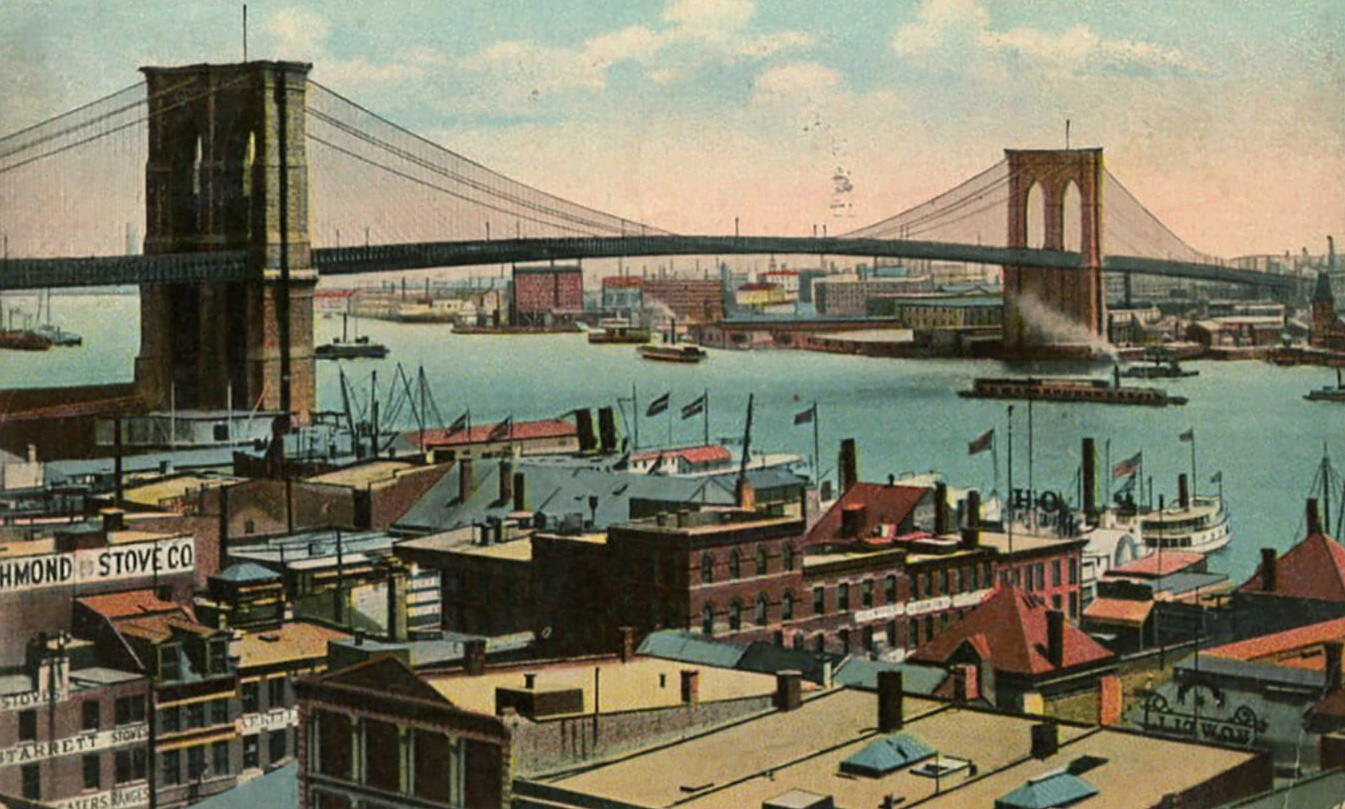
\includegraphics[width=0.9\linewidth]{brooklyn-bridge.jpg}
  % \caption{The Brooklyn Bridge from the South Street Seaport, circa 1890.}
  \caption{从南街海港处看到的布鲁克林大桥(1890 年左右)}
  \label{fig:brooklyn-bridge}
\end{figure}

% The Williamsburg Bridge was not as well maintained as evidenced by its mergency closing in 1988. In April of that year, after a thorough inspection revealed corrosion of the cables, beams and steel supports, the Williamsburg Bridge was closed to all vehicular and train traffic for nearly two months. After engineers performed emergency construction on the bridge and reopened it to traffic, a panel of design experts convened to determine if the Williamsburg Bridge should be replaced, or if it should be rehabilitated. In November 1988, after evaluating several alternatives, the New York City Department of Transportation (DOT) determined that the Williamsburg Bridge should be repaired while kept open to traffic. This option was deemed to have the least detrimental impact on motorists and nearby communities. In 1991, the New York City DOT began a major rehabilitation of the Williamsburg Bridge. The program  was designed to undo the effects of age, weather, increased traffic volumes, and deferred maintenance. \Cref{fig:williamsburg-bridge} shows the Williamsburg Bridge circa 1904.
威廉斯堡大桥在 1988 年进行紧急关闭,这表明其维护得并不好。当年 4 月,在经过彻底检查发现主缆、横梁和钢支承有所腐蚀后,威廉斯堡大桥对所有汽车和火车关闭交通将近两个月。在工程师对桥梁进行紧急施工并重新开放交通后,一个设计专家小组召开会议,以确定是否应该更换威廉斯堡大桥,或者对其进行修复。1988 年 11 月,在评估了几种备选方案后,纽约市\acrfull{dot}决定修复威廉斯堡大桥,同时保持交通畅通。该选项被认为对驾车者和附近社区的不利影响最小。1991 年,纽约市\acrlong{dot}开始启动对威廉斯堡大桥进行大规模修复的计划,该计划旨在消除结构老化、天气、交通量增加和维护延期的影响。 \cref{fig:williamsburg-bridge} 显示了大约 1904 年的威廉斯堡大桥。

\begin{figure}
  \centering
  
\includegraphics[width=0.9\linewidth]{williamsburg-bridge.jpg}
  % \caption{The Williamsburg Bridge, circa 1904.}
  \caption{威廉斯堡大桥(1904 年左右)}
  \label{fig:williamsburg-bridge}
\end{figure}

% The decision to rehabilitate the Williamsburg Bridge instead of undertaking a costly in-place replacement in downtown Manhattan was made possible by the original conservative design of the bridge cables. The need to rehabilitate the cable was necessitated by a poor corrosion-protection choice. Leffert~L. Buck, the designer of the Williamsburg Bridge, chose linseed oil. The 1988 inspection of the Williamsburg Bridge cables revealed significant corrosion, proving the choice of linseed oil to be a relatively poor one. For the Brooklyn Bridge, John Augustus Roebling chose a coating of graphite to protect the individual wires of the bridge cable from corrosion, a choice that provided over 100 years of corrosion protection. Fortunately, the cable design for the Williamsburg Bridge utilized a factor of safety of resistance divided by load of about 5. After the significant loss of section due to corrosion was observed in 1988, the factor of safety was deemed adequate and a cable rehabilitation program to arrest the corrosion was initiated instead of a cable replacement. Thus, original overdesign allowed the bridge and its cables to continue in service.
威廉斯堡大桥采取了修复的方式而不是在曼哈顿市中心进行昂贵的就地更换,这项决定之所以具有可行性,其原因在于桥梁主缆最初采用了保守设计。由于防腐体系的选择不当,主缆需要进行修复。威廉斯堡大桥的设计者 \pnme{Leffert~L. Buck} 在主缆防腐上选择了亚麻籽油。 1988 年对威廉斯堡大桥主缆的检查发现有明显的腐蚀,证明亚麻籽油的选择是一个相对较差的选择。而像布鲁克林大桥,\pnme{John Augustus Roebling} 选择了石墨涂层来保护桥梁主缆的单根钢丝免受腐蚀,这种方案就提供了长达 100 多年的腐蚀保护。幸运的是,威廉斯堡大桥的主缆设计采用了抗力与荷载之比为 5 左右的安全系数。即使在 1988 年观察到由于腐蚀造成的截面显著损失后,其安全系数也被认为是足够的,这样,防止腐蚀的主缆修复计划得以启动,桥梁并没有更换主缆。因此,实际上是最初的过度设计允许桥梁及其主缆继续使用。

% The Eads Bridge, completed in 1874 and named for its designer and builder, James Buchanan Eads, has proven long-lived by being well maintained and readily adaptable. \Cref{fig:eads-bridge} shows the Eads Bridge circa 1983. The scale of the bridge was unprecedented: the more than 500-ft span of the center arch exceeded by some \qty{200}{ft} any arch built previously. The arch ribs were made of steel, its first extensive use in a bridge. An additional innovation was the cantilever erection of the arches without falsework, the first example of this type of construction for a major bridge.

伊兹桥于 1874 年完工,并以其设计师和建造者 \pnme{James Buchanan Eads} 的名字命名,由于自身良好的适应性且经过良好维护,它经久不衰。 \cref{fig:eads-bridge} 显示了大约 1983 年的伊兹桥。这座桥的规模是前所未有的:中心拱 \qty{150}{m} 的跨度超过了以往建造的任何一座拱桥的拱肋跨度(\qty{60}{m}左右)。拱肋采用了桥梁中的首次使用的钢结构拱肋。另一项创新是在无支架的情况下悬臂架设主拱,这是采用此类施工方法建设大型桥梁的第一个例子。

\begin{figure}
  
\includegraphics[width=0.9\linewidth]{eads-bridge.jpg}
  % \caption{The Eads Bridge looking toward St. Louis and the Gateway Arch, circa 1983.}
  \caption{向圣路易斯和拱门方向望去的伊兹桥(1983 年左右)}
  \label{fig:eads-bridge}
\end{figure}

% An interesting feature of the history of the Eads Bridge has been its adaptability to varying use. (It should be noted that the Brooklyn and Williamsburg Bridges have also seen varied use.) The bridge was originally a railway bridge carrying pedestrians on an upper deck with two rail lines below. The Eads Bridge eventually carried vehicular and rail traffic and the last train crossed the bridge in 1974. By the early 1990s, traffic on the bridge had dwindled to about \num{4000} cars a day and in 1991, the Eads Bridge was closed. For a while, it was unused altogether, but in 1993, new uses were found. MetroLink, the region's new light rail system, began to use the lower deck, which originally served passenger and freight train traffic and in 2003, the upper deck reopened to buses and automobiles. Today, a new lane for pedestrians and bicyclists on the south side of the bridge provides a great place to look at the river and the skyline of the city.
有关伊兹桥历史上的一个有趣特征是它对不同用途的适应性。(应该指出的是,布鲁克林大桥和威廉斯堡大桥也有不同的用途。)这座桥最初是一座铁路桥,上层载有行人,下面有两条铁路线。伊兹桥实际上最终承载了车辆和铁路交通,直到最后一列火车于 1974 年通过了这座桥。到 1990 年代初,桥上的交通量减少到每天约 \num{4000} 辆汽车,到了 1991 年,伊兹桥关闭。此后有一段时间内,它完全没有被使用,直到 1993 年,发现了新的用途。该地区的新轻轨系统 MetroLink 开始使用最初服务于客运和货运列车交通的下层,到了 2003 年,上层重新向公共汽车和汽车开放。如今,大桥南侧的行人和自行车道成为了观赏河流和城市天际线的绝佳场所。

% The examples of these three 100-plus yr old bridges illustrates that for bridges to serve a long life, they must be:
这三座历经 100 多年的老桥的例子说明,要使桥梁\gls*{servicelife}更长久,它们必须是:
\begin{itemize}
  % \item Resistant to environmental and man-made hazards,
  \item 具有抵抗环境和人为危害的能力;
  % \item Maintainable (and subsequently maintained) or relatively maintenance-free, and
  \item 具有可维护性(并在随后切实维护)或具有相对免维护性;
  % \item Adaptable to changes in traveled-way cross section and usage.
  \item 对行车道断面和使用用途的变化具有一定的适应性。
\end{itemize}

% Traditional approaches for enhancing the service life of bridges used in various codes and specifications such as AASHTO specifications, Eurocodes, or British Standards, are mainly in an indirect form, specifying the use of certain details or properties such as cover thickness, maximum crack width, concrete compressive strength, etc.
\acrshort{aashto} 规范、欧洲规范或英国标准等各种规范中使用的提高桥梁\gls*{servicelife}的传统方法主要采用间接方式,即指定使用某些细节或属性,例如保护层厚度、最大裂缝宽度、混凝土抗压强度等。

% Recognizing the importance of design for service life has motivated different agencies to undertake new initiatives for developing more formal design approaches for service life, similar to those used for design for strength. However, to date the majority of these efforts have concentrated on addressing concrete durability and service life, and significant advances have been achieved in this field. Designing bridges for service life, however, is more than just addressing service life and durability of concrete.

认识到\gls*{servicelife}设计的重要性促使不同的机构采取新的举措来开发更正式的\gls{servicelife}设计方法,类似于用于强度设计的方法。迄今为止,这些努力中的大部分都集中在解决混凝土的耐久性和\gls*{servicelife}问题上,并且在该领域已经取得了重大进展。然而,为\gls*{servicelife}设计桥梁不仅仅是解决混凝土的\gls*{servicelife}和耐久性问题。

% Furthermore, the design for service life for bridges needs to be approached in a systematic, all-inclusive manner rather than as a series of isolated tasks, each addressing service life of a particular portion of a bridge independently. The interaction between strategies for enhancing the service life of different bridge elements, components, and subsystems must be given critical consideration. In addition, a maintenance program, retrofit or replacement options, and management plan should all be part of this systematic service life design approach. In summary, at the design stage the design for service life should be approached as a comprehensive plan capable of providing the owner with a complete picture of what will be necessary for the bridge to achieve its specified service life.
此外,桥梁的\gls*{servicelife}设计需要以系统的、包罗万象的方式进行,而不是作为一系列孤立的任务,每个任务都独立地处理桥梁特定部分的\gls*{servicelife}。必须严格考虑提高不同桥梁\gls*{element}、\gls*{component}和\gls*{subsystem}\gls*{servicelife}的措施之间的相互作用。此外,维护计划、改造或更换选项以及管理计划都应该是该系统\gls*{servicelife}设计方法的一部分。总而言之,在设计阶段,\gls*{servicelife}设计应作为一个综合计划来处理,该计划能够为业主提供一个完整的画面,说明桥梁达到其指定\gls*{servicelife}所需的条件。

% The most notable efforts to develop a scientific approach for service life and durability of concrete elements (covering buildings, bridges, and tunnels) were a series of studies carried out between 1996 and 1999 in Europe for the fédération international du béton (The International Federation for Structural Concrete). One of the products of these efforts was the publication of \textbf{\em fib} \bkn{Bulletin 34}, \emph{Model Code for Service Life Design}, (TTD 2006). \emph{Bulletin 34}, however, only concentrated on addressing concrete service life and durability. Further, caution must be exercised when applying the recommendations of this publication to concrete placed in a horizontal configuration, such as a bridge decks. While \emph{Bulletin 34} has many useful recommendations for designing concrete elements for service life and  durability, the application of these recommendations to bridge components such as bridge decks remains a point of debate (in particular the use of various solutions to Fick's second law to predict the rate of chloride ingress through deck concrete). The use of recommendations made in \emph{Bulletin 34} is believed to be most applicable for concrete in vertical configuration and under compression, such as in substructure columns or sides of concrete box girders. This same debate can also be extended to the use of some of the available commercial and noncommercial programs that use the fundamental concepts stated in \bkn{Bulletin 34}.
科研人员为开发科学的方法来提高混凝土构件(包括建筑物、桥梁和隧道)的\gls*{servicelife}和耐久性做出了很多努力,其中最引人注目的是\acrfull{fib}于 1996 年至 1999 年间在欧洲进行的一系列研究。其成果之一是发布了\bkn*{\acrshort*{fib} Bulletin 34, Model Code for Service Life Design} \cite{fib2006}。然而,\bkn*{Bulletin 34} 只专注于解决混凝土的\gls*{servicelife}和耐久性问题。此外,在将其建议应用于水平设置的混凝土(例如桥面板)时,必须谨慎行事。虽然 \bkn*{Bulletin 34} 对设计混凝土构件的\gls*{servicelife}和耐久性提出了许多有用的建议,但将这些建议应用于桥面系等桥梁\gls*{component}仍然是一个争论点(特别是在使用各种解决方案来解决菲克第二定律预测氯离子在桥面板混凝土中的渗透速度方面)。\bkn*{Bulletin 34} 中提出的建议被认为最适用于垂直设置和受压的混凝土,例如子结构柱或混凝土箱梁的侧面。同样的争论也可以扩展到一些使用 \bkn*{Bulletin 34} 中陈述的基本概念的商业和非商业程序的使用。

% Efforts to address service life of bridges are not limited to Europe. A significant number of research studies have been and are presently (2012) being carried out to develop solutions for various service life issues related to different bridge types.
解决桥梁\gls*{servicelife}问题的努力并不局限于欧洲。目前(2012 年)大量研究已经进行或正在进行中,这些研究针对不同桥梁类型的\gls*{servicelife}问题开发解决方案。

% One of the missing elements for designing bridges for service life is the framework that would approach the problem in a systematic manner and provide a complete solution in a format that could ensure long lasting bridges. Individual solutions to issues that historically have reduced service life, maintenance plans, retrofit or replacement plans, bridge management, and life cycle cost analysis are all just components of this systematic framework and not the framework itself. The steps within this framework should start at the design stage and should provide the owner with complete information for ensuring the serviceability of the bridge for a specified target service life. It is important for the plan to be transparent and identify the challenges for the period of specified service life, at the design stage, so that the owner will encounter no surprises.

实施桥梁\gls*{servicelife}设计所缺少的要素之一是一个系统框架,该框架是以系统的方式处理问题并提供格式化的完整解决方案来保证桥梁的耐久性。针对历史上造成缩短\gls*{servicelife}问题的单独解决方案、维护计划、改造或更换计划、桥梁管理和\acrlong*{lcca}都只是该系统框架的组成部分,而不是框架本身。该框架内的步骤应从设计阶段开始,并应为业主提供完整的信息,以确保桥梁在特定目标\gls*{servicelife}内的适用性。重要的是计划要透明,并在设计阶段确定在指定\gls*{servicelife}期间面临的挑战,这样业主就不会遇到意外。

% \section{Objectives of the Guide}
\section{《指南》的目标}
% The main objective of the Guide is to provide information about, and define procedures for systematically designing for service life and durability for both new and existing bridges. The cost of addressing service life issues at the design stage is significantly lower than taking maintenance and reservation actions while the bridge is in service.
\bkn{指南}的主要目标是提供有关新旧桥梁\gls*{servicelife}和耐久性的系统性设计的信息并为之定义程序。在设计阶段解决\gls*{servicelife}问题的成本明显低于在桥梁使用期间采取维护和保留措施的成本。

% \section{Bridge Service Life Related Terminology and Relationships}
\section{桥梁\glsentrytext{servicelife}相关术语和关系}\label{sec:BSL-terminology-relationship}
% The following sections provide service life related terminology and relationships used in the Guide.
以下部分提供了\bkn{指南}中使用的与\gls*{servicelife}相关的术语和关系。

% \subsection{Service Life and Design Life}
\subsection{\glsentrytext{servicelife}与\glsentrytext{designlife}}
\begin{description}[style=nextline,leftmargin=10.5em]
  % \item[Service Life.] The time duration during which the bridge element, component, subsystem, or system provides the desired level of performance or functionality, with any required level of repair and/or maintenance.
  \item[\gls{servicelife}] \glsdesc{servicelife}。
  % \item[Target Design Service Life.] The time duration during which the bridge element, component, subsystem, and system is expected to provide the desired function with a specified level of maintenance established at the design or retrofit stage.
  \item[\gls{targetdesignservicelife}] \glsdesc{targetdesignservicelife}。
  % \item[Design Life.] The period of time on which the statistical derivation of transient loads is based: 75 years for the current version of \emph{AASHTO LRFD Bridge Design Specifications} (2012), hereafter referred to as \emph{LRFD Specifications}. 
  \item[\gls{designlife}] \glsdesc{designlife},根据现行的 \bkn*{AASHTO LRFD Bridge Design Specifications (2012)}(以下简称 \lrfd)为 75 年。
\end{description}

% \subsection{Bridge Element, Component, Subsystem, and System}
\subsection{桥梁\glsentrytext{element}、\glsentrytext{component}、\glsentrytext{subsystem}与\glsentrytext{system}}
% The term bridge subsystem is introduced by the Guide. The terms bridge element, component, and system are the same as that defined by FHWA National Bridge Inventory.
术语\gls{subsystem}由\bkn{指南}引入。术语桥梁\gls{element}、\gls{component}和\gls{system}与\gls{fhwa}国家桥梁清单定义的相同。

\begin{description}[style=nextline,leftmargin=7.5em]
  % \item [Bridge Element] Individual bridge members such as a girder, floor beam, stringer, cap, bearing, expansion joint, railing, etc. Combined, these elements form subsystems and components, which then constitute a bridge system.
  \item [桥梁\gls{element}] \glsdesc*{element}。
  % \item [Bridge Component] A combination of bridge elements forming one of the three major portions of a bridge that makes up the entire structure. The three major components of a bridge system are substructure, superstructure, and deck.
  \item [桥梁\gls{component}] \glsdesc*{component}。
  % \item [Bridge Subsystem] A combination of two or more bridge elements acting together to serve a common structural purpose. Examples include composite girder, which could consist of girder, reinforcement, and concrete.
  \item [桥梁\gls{subsystem}] \glsdesc*{subsystem}。
  % \item [Bridge System] The three major components of the bridge—deck, substructure and superstructure—combined to form a complete bridge.
  \item [桥梁\gls{system}] \glsdesc*{system}。
\end{description}

% \subsection{Service and Design Life: Basic Relationships}
\subsection{\glsentrytext{servicelife}与\glsentrytext{designlife}的基本关系}

% Several basic relationships exist between service lives of bridge components, elements, subsystems and systems, and bridge design life. Following are descriptions of these relationships.

桥梁\gls*{element}、\gls*{component}、\gls*{subsystem}和\gls*{system}的\gls*{servicelife}与桥梁\gls*{designlife}之间存在几种基本关系。以下是对这些关系的描述。

\begin{itemize}
  % \item Predicting service life of bridge systems is accomplished by predicting service life of its elements, components, or subsystems.
  \item 预测桥梁\gls*{system}的\gls*{servicelife}是通过预测其\gls*{element}、\gls*{component}和\gls*{subsystem}的\gls*{servicelife}来完成的。
  % \item The design life of a bridge system is a target life in years, set at the initial design stage and specified by the bridge owner.
  \item 桥梁\gls*{system}的\gls*{designlife}是以年为单位的目标寿命,在最初设计阶段由业主指定。
  % \item The service life of a given bridge element, component, subsystem, or system could be more than the target design service life of the bridge system.
  \item 给定的桥梁\gls*{element}、\gls*{component}、\gls*{subsystem}或\gls*{system}的\gls*{servicelife}可以比桥梁\gls*{system}的\gls*{targetdesignservicelife}更长。
  % \item The end of service life for a bridge element, component, or subsystem does not necessarily signify the end of bridge system service life as long as the bridge element, component, or subsystem could be replaced or resume its function with retrofit.
  \item 桥梁\gls*{element}、\gls*{component}或\gls*{subsystem}达到\gls*{servicelife}并不一定意味着桥梁\gls*{system}也达到了\gls*{servicelife},只要桥梁\gls*{element}、\gls*{component}或\gls*{subsystem}可以更换并通过改造恢复其功能即可。
  % \item A given bridge element, component, or subsystem could be replaced or retrofitted, allowing the bridge as a system to continue providing the desired function.
  \item 可以通过更换或改装给定的桥梁\gls*{element}、\gls*{component}或\gls*{subsystem},使桥梁作为一个\gls*{system}继续提供所需的功能。
  % \item The service life of a bridge element, component, or subsystem ends when it is no longer economical or feasible to repair or retrofit it, and replacement is the only remaining option.
  \item 当桥梁\gls*{element}、\gls*{component}或\gls*{subsystem}的维修或改造不再具有经济性或不具备可行性时,其\gls*{servicelife}就结束了,更换是剩下的唯一选择。
  % \item The service life of a bridge system ends when it is not possible to replace or retrofit one or more of its components, elements, or subsystems economically or because of other considerations.
  \item 当从经济性上或出于其他考虑无法更换或改造其一个或多个\gls*{element}、\gls*{component}或\gls*{subsystem}时,桥梁\gls*{system}的\gls*{servicelife}结束。
  % \item The service life of a bridge system is governed by the service life of its critical elements, components, and subsystems. The critical bridge elements, components, or subsystems are defined as those needed for the bridge as a system to provide its intended function.
  \item 桥梁\gls*{system}的\gls*{servicelife}取决于其关键\gls*{element}、\gls*{component}和\gls*{subsystem}的\gls*{servicelife}。桥梁\emph{关键\gls*{element}、\gls*{component}和\gls*{subsystem}}的定义是:为桥梁作为一个\gls*{system}提供其预期功能所需的那些\gls*{element}、\gls*{component}和\gls*{subsystem}。
\end{itemize}

% In general, the service life, $t_\text{s}$ , of the bridge elements, components, and subsystems should be equal to or greater than the design life, $t_\text{D}$ of the bridge system defined by Equation 1.1.
一般来说,桥梁\gls*{element}、\gls*{component}和\gls*{subsystem}的\gls*{servicelife} $t_\text{s}$ 应大于等于桥梁\gls*{system}的\gls*{designlife} $t_\text{D}$,如\cref{eq:system-design-life-vs-element-service-life} 所示。
\begin{equation}
  \label{eq:system-design-life-vs-element-service-life}
  \left( t_\text{s}\right)_\text{C,E,SS} \geqslant \left( t_\text{D}\right)_\text{BS}
\end{equation}
\begin{EqDesc}{\left( t_\text{s}\right)_\text{C,E,SS}}
  \item[\left( t_\text{s}\right)_\text{C,E,SS}] 桥梁\gls*{component}(C)、\gls*{element}(E)或\gls*{subsystem}(SS)的\gls*{servicelife};
  \item[\left( t_\text{D}\right)_\text{BS}] 桥梁\gls*{system}的\gls*{designlife}。
\end{EqDesc}

% The service life of the bridge system is less than or equal to the service life of its governing elements, components or subsystems, as described by Equation 1.2.
桥梁\gls*{system}的\gls*{servicelife}要小于等于其控制性\gls*{element}、\gls*{component}或\gls*{subsystem}的\gls*{servicelife},如\cref{eq:system-service-life-vs-key-element-service-life} 所示:
\begin{equation}
  \label{eq:system-service-life-vs-key-element-service-life}
  \left( t_\text{s}\right)_\text{BS} \leqslant \left[ \left( t_\text{s}\right)_\text{C,E,SS} \right]_\text{critical}
\end{equation}

% The service life of the bridge system must exceed or be equal to the target design life of the bridge system as described by Equation 1.3.
桥梁\gls*{system}的\gls*{servicelife}必须大于等于桥梁\gls*{system}的\gls*{targetdesignservicelife},如\cref{eq:system-service-life-vs-system-target-service-life} 所示:
\begin{equation}
  \label{eq:system-service-life-vs-system-target-service-life}
  \left( t_\text{s}\right)_\text{BS} \geqslant \left( t_\text{D}\right)_\text{BS}
\end{equation}

% \section{Guide Approach to Design for Service Life}
\section{《指南》的\glsentrytext{servicelife}设计方法}\label{sec:guide-approach}
% The Guide approach to design for service life is to provide a body of knowledge relating to bridge durability under different exposure conditions and constraints, and to establish an array of options capable of enhancing service life. A solution for a particular service life issue is highly dependent on many factors that vary from location to location and state to state. A solution also depends on local practices and preferences. Consequently, use of the Guide is not intended to dictate a unique solution for any specific service life problem or identify the “best and only” solution. Rather it equips the reader with a body of knowledge for developing specific solutions best suited to stated conditions and constraints.
\bkn{指南}的\gls*{servicelife}设计方法是:提供与桥梁在不同暴露条件和约束下的耐久性相关的知识体系,并建立一系列能够延长\gls*{servicelife}的选项。针对特定\gls*{servicelife}问题的解决方案高度依赖于因地点而异的许多因素,同时还取决于当地的做法和偏好。因此,\bkn{指南}的使用并非旨在为任何特定的\gls*{servicelife}问题规定“最佳且唯一”的解决方案。相反,它为读者提供了开发最适合规定约束条件的特定解决方案的知识体系。

% In applying the Guide framework to a particular bridge, including long-span bridges, an array of solutions can be identified for enhancing the service life of a the bridge element, component, or subsystem, and an optimum solution can be identified through life cycle cost analysis. The solutions can be based on data collected by local DOTs or agencies responsible for maintaining the bridge and, in order to be complete, the life cycle cost analysis should include maintenance, retrofit, replacement, and user costs. It is important that the list of assumptions and feasible solutions considered for a particular bridge element, component, and subsystem be communicated and shared with the owner, especially with respect to the life cycle cost analysis, so that the entire process is fully transparent.
在将\bkn{指南}框架应用于特定桥梁(包括大跨度桥梁)时,可以确定一系列解决方案以提高桥梁\gls*{element}、\gls*{component}或\gls*{subsystem}的\gls*{servicelife},并且可以通过\acrlong*{lcca}确定最佳解决方案。解决方案可以基于当地\acrlong*{dot}或负责维护桥梁的机构收集的数据,并且为了完整,\acrlong*{lcca}应包括维护、改造、更换和用户成本。重要的是要与业主沟通和共享针对特定桥梁\gls*{element}、\gls*{component}和\gls*{subsystem}考虑的假设和可行解决方案列表,尤其是在\acrlong*{lcca}方面,这可以使整个过程完全透明。

% The Guide recognizes that not all bridges can or need to have 100 years of service life. Therefore maintenance, rehabilitation, and replacement are part of the service life design process. The Guide provides the general framework to achieve this objective in a systematic manner that considers the entire bridge system and all project demands.
\bkn{指南}认识到并非所有桥梁都可以或需要有 100 年的\gls*{servicelife}。因此,维护、修复和更换是\gls*{servicelife}设计过程的一部分。\bkn{指南}考虑了整个桥梁\gls*{system}和所有项目需求,提供了以系统方式实现这一目标的总体框架。

% There are different ways of achieving enhanced service life of existing and new bridges. Two examples include using improved, more durable materials and systems during original construction that will require minimal maintenance, and improving techniques and optimizing the timing of interventions such as preventive maintenance actions. Interventions can be planned and carried out based on the assessment of individual bridge conditions and needs, or based on a program of preventive maintenance actions planned for similar elements on a group of bridges. A simple example of a preventive, planned maintenance program might include the following activities:
有不同的方法可以延长既有桥梁和新建桥梁的\gls{servicelife}。举两个例子,其一是在初始施工期间使用改进的、耐用的材料和\gls*{system},这将需要最少的维护;另一种可能是改进技术和优化预防性维护行动这类干预措施的实施时间。可以根据对个别桥梁状况和需求的评估,或根据为一组桥梁上同类\gls{element}而计划的预防性维护程序,来规划和实施干预措施。举一个简单的例子,预防性、有计划的维护程序可能包括以下活动:

% \begin{itemize}
  % \item Washing deicing salts off bridge decks in the spring,
  % \item Cleaning debris from bridge deck expansion joints,
  % \item Cleaning debris from bearings and truss joints,
  % \item Cleaning drainage outlets,
  % \item Spot painting steel structures
  % \item Sealing decks or superstructures in marine environments, and
  % \item Sealing substructures on overpasses where deicing salts are used on the roadways below.
% \end{itemize}
\begin{itemize}
  \item 春天清洗桥面上的除冰盐;
  \item 清理桥面伸缩缝内的杂物;
  \item 清除支座和桁架节点上的杂物;
  \item 清洗排水口;
  \item 涂装钢结构;
  \item 封闭海洋环境中的桥面系​​或上部结构;
  \item 封闭处于使用除冰盐的地面道路上的立交桥下部结构。
\end{itemize}

% By acknowledging that service life can be extended by either using more durable, deterioration-resistant materials or by planned intervention, a cost comparison can be made to determine the most cost effective approach for various environmental exposure levels and various levels of available maintenance and preservation actions.
使用抗\gls*{deterioration}的耐用材料或通过有计划的干预可以延长\gls*{servicelife},承认这一事实,就可以进行成本比较,从而确定针对各种环境暴露水平和各种可用维护和保护措施水平的最具成本效益的方法。

% The following sections provide an overview of the general approach used in the Guide. The discussion is customized for new bridges; however, use of the Guide approach for existing bridges can be accomplished by eliminating some of the steps that are used for new bridges. Because the discussions are general and use very simple examples to demonstrate the point of discussion many intermediate steps are eliminated for the sake of clarity. More detailed procedures and examples are provided in subsequent chapters of the Guide.
以下各节概述了\bkn{指南}中使用的一般方法。讨论是为新建桥梁定制的;然而,对既有桥梁来说,只要取消一些专门用于新建桥梁的步骤即可。由于讨论是笼统的,并且使用非常简单的示例来说明讨论的要点,因此为了清楚起见,省略了许多中间步骤。\bkn{指南}的后续章节提供了更详细的程序和示例。

% Three related flowcharts, as shown in Figures 1.4, 1.5 and 1.6, are used to demonstrate the general approach used in the Guide. Blocks within each flowchart are numbered. Following each flowchart, a brief discussion explains the intent of each block within that flowchart.
如\cref{fig:general-flowchart} 所示的流程图用于演示\bkn{指南}中使用的一般方法。流程图中的模块都已编号,并简短的讨论解释了流程图中每个模块的涵义。

% It should be noted that customization of the framework introduced in the Guide for a particular bridge could be achieved by developing similar flowcharts, making each step of the process transparent to the owner. For major and complex bridges, various elements of the flowcharts need to reflect specific project requirements.
应该注意的是,\bkn{指南}中为特定桥梁引入的框架定制可以通过开发类似的流程图来实现,使过程的每个步骤对业主透明。对于主要和复杂的桥梁,流程图的各种元素需要反映特定的项目要求。

% The sections that accompany Figures 1.4, 1.5 and 1.6 describe elements within the flowcharts. Each block within the flowcharts is numbered and described under the corresponding Step number. For example, Step 1 corresponds to block number 1 in \cref{fig:general-flowchart}.
\cref{fig:general-flowchart} 的相关部分描述了流程图\footnote{译者将原文中的三张流程图合成了一张总流程图。}中的元素。流程图中的每个模块都在相应的步骤编号下进行了编号和描述。例如,步骤 1 对应于\cref{fig:general-flowchart} 中的模块号 1。

\begin{figure}
  % 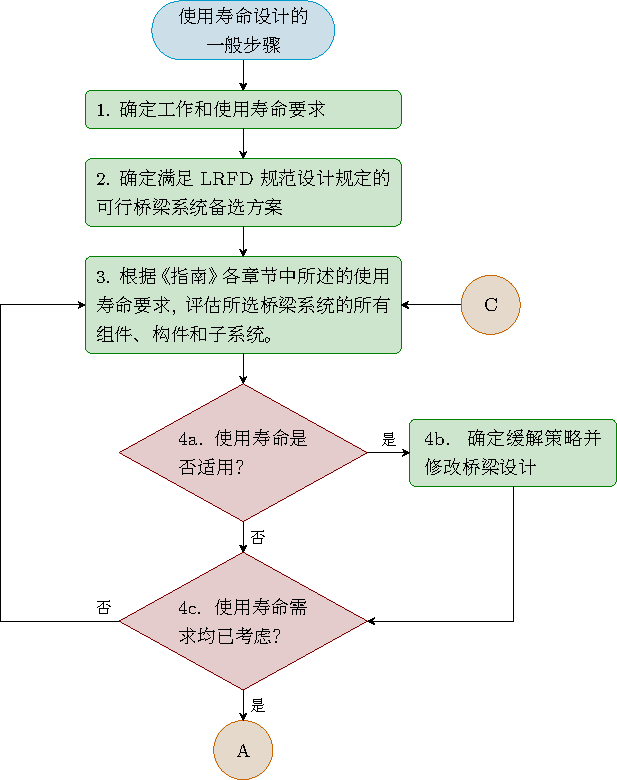
\includegraphics{flowcharta.pdf}
  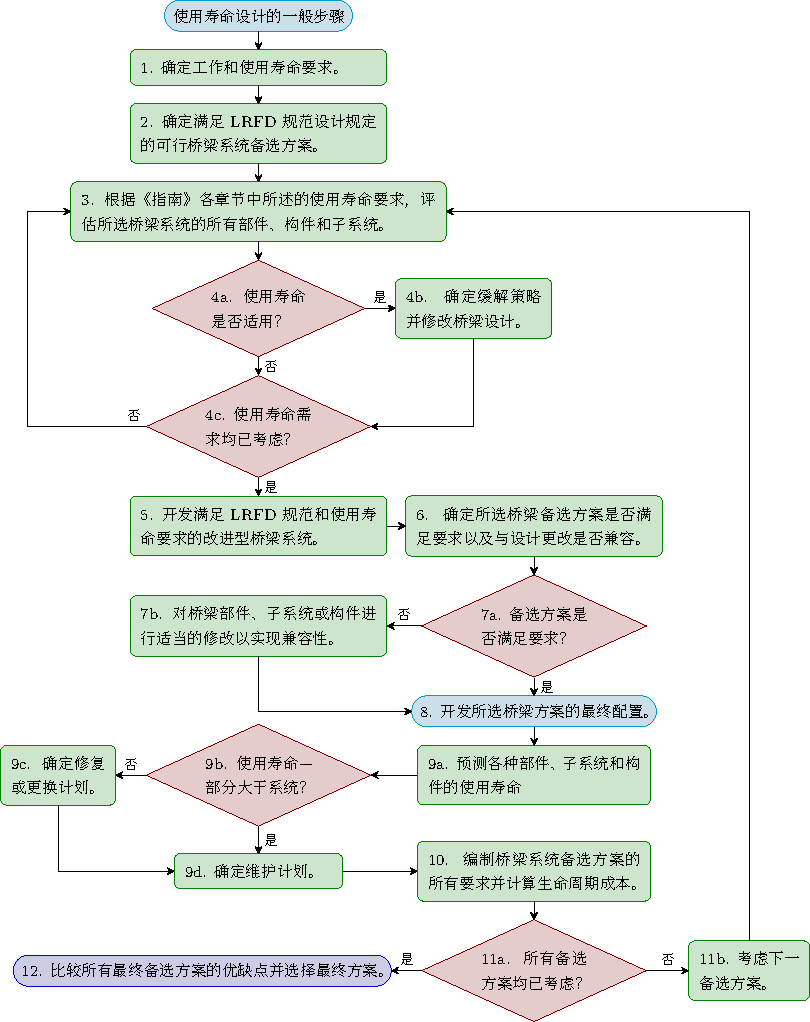
\includegraphics{flowchart.pdf}
  \caption{展示\bkn{指南}的\gls{servicelife}设计方法的总流程图}
  \label{fig:general-flowchart}
\end{figure}

  % \emph{Step 1.} The design for service life starts by first considering all project demands set by the owner, including the service life requirements, as stated in \cref{fig:general-flowchart}. \cref{chp:bridge-system-selection} provides examples of local operational and site requirements, as well as service life considerations, needing attention.
\emph{步骤 1}\quad \gls*{servicelife}设计首先考虑业主设定的所有项目需求,包括\gls{servicelife}要求,如\cref{fig:general-flowchart} 中所述。\cref{chp:bridge-system-selection}提供了本地操作和现场要求的示例,以及\gls{servicelife}注意事项,需要注意。
  
% \emph{Step 2.} Develop all feasible and preliminary bridge alternatives that satisfy project demands. For example, one might want to consider steel, concrete, and segmental bridge alternates for a particular bridge. The development of the potential bridge systems is carried out in a conventional manner, meeting all the provisions of the LRFD Specifications. It is good practice to consider potential service life problems, even at this stage of the design process. It is also feasible to use bridge technologies which do not have a specific design guideline within the LRFD Specifications. In such cases, the best available design approach could be used, subject to owner approval.
\emph{步骤 2}\quad 开发满足项目需求的所有可行和初步的桥梁备选方案。例如,人们可能想要在某特定桥梁的设计中考虑钢、混凝土和节段桥方案。潜在桥梁\gls*{system}的开发以传统方式进行,满足 \lrfd 的所有规定。优良作法是考虑潜在的\gls*{servicelife}问题,即使在设计过程的这个阶段也是如此。使用 \lrfd 中没有特定设计指南的桥梁技术也是可行的。在这种情况下,可以使用最佳可用设计方法,但须经业主批准。

  % \emph{Step 3 to 4} The next step in the process consists of evaluating each bridge system alternate one at a time and considering service life issues related to each element, component, and subsystem of that bridge system. For each bridge element, component, and subsystem, the Guide provides a framework for incorporating the changes and modifications needed to meet service life requirements.
\emph{步骤 3~4}\quad 该过程接下来的一步包括一次评估每个桥梁\gls*{system},并考虑与该桥梁\gls*{system}的每个\gls*{element}、\gls*{component}和\gls*{subsystem}相关的\gls*{servicelife}问题。对于每个桥梁\gls*{element}、\gls*{component}和\gls*{subsystem},该指南提供了一个框架,用于合并满足\gls*{servicelife}要求所需的更改和修改。

% For example, assume that one of the bridge systems to be considered for a particular project is a steel bridge alternate. The designer will first develop the preliminary bridge configurations using the conventional approaches that meet all LRFD Specifications. Then, using procedures depicted in blocks 4a, 4b, 4c, each element, component, or subsystem of the steel alternate will be checked against the service life requirements using the fault tree approach described later in the Guide. These evaluation requirements may lead to changes in the details of the element, component, or subsystem under consideration. For example, the preliminary deck configuration may indicate that use of 8-in. thick concrete is sufficient from a strength standpoint. Going through the fault tree corresponding to bridge deck and described in Chapter 4 of the Guide, the designer may change the deck thickness to 9 in. to address potential overloads, or may specify sealing the bottom of the deck to protect it from salt spray, if the bridge is located along the coastline. It should be noted that for major and complex bridges, most of these fault trees must be customized to meet specific needs and preferred practices. Examples of fault trees and how they work are provided in later sections of this chapter.
例如,假设要为特定项目考虑的桥梁\gls*{system}的备选方案之一是钢桥方案。设计人员将首先使用满足所有 \lrfd 的传统方法进行初步的桥梁设计。然后,使用模块 4a、4b、4c 中描述的程序,将使用\bkn{指南}后面描述的\gls*{faulttree}方法根据\gls*{servicelife}要求检查钢桥方案的每个\gls*{element}、\gls*{component}或\gls*{subsystem}。这些评估要求可能导致正在考虑的\gls*{element}、\gls*{component}或\gls*{subsystem}的细节发生变化。例如,从强度的角度来看,桥面板最初设计使用 \qty{20}{cm} 厚的混凝土就足够了,通过与\bkn{指南}\cref{chp:bridge-decks}中描述的桥面板对应的\gls*{faulttree},设计者可以将桥面板厚度更改为 \qty{23}{cm} 以解决潜在的超载问题,或者如果桥梁位于海岸线上,则可以指定密封桥面板底部以防止盐雾影响。应该注意的是,对于大型和复杂的桥梁,这些\gls*{faulttree}中的大多数必须定制以满足特定需求和首选实践。本章后面的部分提供了\gls*{faulttree}示例及其工作原理。

% \emph{Step 5 to 8} At the end of Step 4 and after going through appropriate fault trees for various bridge elements, components, and subsystems, the designer will have developed a bridge system that meets both strength and service life requirements, as illustrated by Step 5 in Figure 1.5. To some extent, changes to configurations of various bridge elements, components, and subsystems are carried out separately. Therefore there is a need to make sure that these changes are compatible and not contradictory or overly conservative. Steps 6 and 7 in Figure 1.5 depict this process. For example, in the steel bridge example discussed previously, service life requirements may dictate the use of a jointless, integral abutment system and require metalizing the end of the girder. The designer may then want to consider not metalizing the end of the girder, since leaking joints would be eliminated. Finally, for the selected bridge system alternate under consideration a final configuration is developed, Step 8, that meets both strength and service life requirements.
\emph{步骤 5~8}\quad 在步骤 4 结束时,在为各种\gls*{element}、\gls*{component}和\gls*{subsystem}查看适当的\gls*{faulttree}后,设计者将设计出满足强度和\gls*{servicelife}要求的桥梁\gls*{system},如\cref{fig:general-flowchart} 中的步骤 5 所示。在某种程度上,各种桥梁\gls*{element}、\gls*{component}和\gls*{subsystem}的配置更改是分开进行的。因此,需要确保这些变化是兼容的,而不是相互矛盾或过于保守的。\cref{fig:general-flowchart} 中的步骤 6 和步骤 7 描述了这个过程。例如,在前面讨论的钢桥方案的例子中,\gls*{servicelife}要求可能要求使用无缝的整体桥台系统,并且需要对大梁的末端进行金属化处理。设计师可能会考虑不对大梁的端部进行金属化处理,因为这样会消除泄漏的接头。最后,对于正在考虑中的选定桥梁\gls*{system}备选方案,将开发最终配置,即第 8 步,以满足强度和\gls*{servicelife}要求。

% \emph{Step 9 to 12} The next step in the process is to evaluate the service life of the various bridge elements, components, and subsystems of the bridge alternate under consideration and compare it to the ownerspecified target service design life of the bridge system. For example, the owner may require that the bridge provide 100 years of service life, whereas the life of a particular bridge element, such as the sliding surface for a bearing, may be limited to 20 years. There would therefore be a need to think ahead and accommodate replacement of the sliding surfaces. Regardless, there will be a need for a systematic maintenance plan that could require the designer to identify “hot areas” requiring more detailed inspection and maintenance. Blocks 9a through 9d depict the development of a maintenance plan and/or rehabilitation and replacement plan for the bridge system alternate under consideration. The result of this process, as illustrated in Step 10, is a bridge system alternate that meets both strength and service life requirements with an associated maintenance and/or rehabilitation or replacement plan for the bridge. The next step, as illustrated in Step 10, is to carry out life cycle cost analysis considering the final configuration of the select bridge alternate and maintenance plan. The same steps are repeated for all bridge alternate systems as shown by Step 11. After comparing all alternates, the designer can then make a recommendation as to which alternate should be used, allowing the owner to make the final selection.
\emph{步骤 9~12}\quad 该过程接下来的一步是评估所考虑的桥梁备选方案的各种桥梁\gls*{element}、\gls*{component}和\gls*{subsystem}的\gls*{servicelife},并将其与业主指定的桥梁\gls*{system}目标服务设计寿命进行比较。例如,业主可能要求桥梁提供 100 年的\gls*{servicelife},而特定桥梁\gls*{element}(例如支座的滑动面)的寿命可能限制为 20 年。因此,需要提前考虑并适应滑动表面的更换。无论如何,都需要一个系统的维护计划,这可能要求设计人员识别需要更详细检查和维护的“热点区域”。块 9a 到 9d 描述了正在考虑的桥梁\gls*{system}备选方案的维护计划和/或修复和更换计划的制定。如步骤 10 所示,此过程的结果是一个桥梁\gls*{system}备选方案,它满足强度和\gls*{servicelife}要求以及相关的桥梁维护和/或修复或更换计划。下一步,如第 10 步所示,是在考虑所选桥梁备选方案和维护计划的最终配置的情况下进行生命周期成本分析。如步骤 11 所示,对所有桥梁备选\gls*{system}重复相同的步骤。在比较所有备选方案后,设计人员可以就应使用哪个备选方案提出建议,让业主做出最终选择。

% As described, the selection of the final bridge system within the framework promoted in the Guide is mainly based on service life requirements. Some of the details included in the steps presented, such as fault tree analysis, will be described in later sections of this chapter.
如前所述,\bkn{指南}所提倡的框架内最终桥梁\gls*{system}的选择主要基于\gls*{servicelife}要求。所介绍的步骤中包含的一些细节,例如\gls*{faulttree}分析,将在本章后面的章节中进行描述。

% A summary of steps for design for service life is provided in \cref{sec:summary-steps} of this chapter.
本章的\cref{sec:summary-steps}中提供了\gls*{servicelife}设计步骤的总结。

% \section{Organization of the Guide}
\section{《指南》的编排组织}

% Included in the Guide are 11 chapters, each devoted to particular bridge elements, components, subsystems, or systems. The following is a brief description of information included in each chapter.
本\bkn{指南}包括 11 章,每章专门介绍特定的桥梁\gls*{element}、\gls*{component}、\gls*{subsystem}或\gls*{system}。以下是对每一章中包含的信息的简要说明。

% \cref{chp:general-frame} \nameref{chp:general-frame} This chapter provides an overview of the approach usedin the Guide for design for service life and describes terminology used throughout the Guide and various relationships that exist between service life of bridge element, component, subsystem, and system and bridge design life as used in AASHTO Specifications. The chapter provides an introduction to the different philosophies used to predict service life.
\cref{chp:general-frame} \nameref{chp:general-frame} 这一章概述了\bkn{指南}中使用的\gls*{servicelife}设计方法,并描述了指南中使用的术语以及桥梁\gls*{element}、\gls*{component}、\gls*{subsystem}和\gls*{system}的\gls*{servicelife}与 \lrfd 中使用的桥梁\gls*{designlife}之间的各种关系。这一章还介绍了用于预测\gls*{servicelife}的不同理论。

% \cref{chp:bridge-system-selection} \nameref{chp:bridge-system-selection} This chapter provides a description of various bridge systems and factors that affect their service life. Included is a description of a general strategy and rational procedure for selecting the optimum bridge system, subsystems, components, and elements, considering specific project limitations and requirements, such as climate, traffic, usage, and importance.

\cref{chp:bridge-system-selection} \nameref{chp:bridge-system-selection} 这一章描述了各种桥梁\gls*{system}以及影响其\gls*{servicelife}的因素。包括对选择最佳桥梁\gls*{system}、\gls*{subsystem}、\gls*{component}和\gls*{element}的一般策略和合理程序的描述,同时考虑特定项目的限制和要求,例如气候、交通、使用和重要性。

% \cref{chp:materials} \nameref{chp:materials} This chapter provides general properties and durability characteristics of the two most commonly used materials in bridge systems, steel and concrete. For each material, a general description of variables affecting the service life is provided, followed by strategies used to mitigate them. \cref{chp:materials} forms the basis for materials used in bridge subsystems and elements specifically addressed in other chapters of the Guide.
\cref{chp:materials} \nameref{chp:materials} 这一章介绍了桥梁\gls{system}中两种最常用的材料(钢材和混凝土)的一般特性和耐久性特征。对于每种材料,提供了影响\gls{servicelife}的变量的一般描述,然后是用于减轻这些变量影响的策略。 \cref{chp:materials} 构成了\bkn{指南}其他章节中特别提到的桥梁\gls{subsystem}和\gls{element}中所使用材料的基础。

% \cref{chp:bridge-decks} \nameref{chp:bridge-decks} This chapter provides descriptions of various bridge deck types and essential information related to their service life, such as modes of deterioration and strategies to mitigate them. The chapter concentrates on cast-in-place and precast concrete bridge decks.
\cref{chp:bridge-decks} \nameref{chp:bridge-decks} 这一章介绍了各种桥面板类型以及与其\gls{servicelife}相关的基本信息,例如\gls*{deterioration}模式和缓解策略。本章重点介绍现浇和预制混凝土桥面板。

% \cref{chp:corrosion-of-steel-rc-bridge} \nameref{chp:corrosion-of-steel-rc-bridge} This chapter looks at basic mechanisms causing corrosion of reinforcement embedded in concrete and provides strategies for preventing corrosion of reinforcement in concrete bridges.
\cref{chp:corrosion-of-steel-rc-bridge} \nameref{chp:corrosion-of-steel-rc-bridge} 这一章着眼于引起混凝土中钢筋腐蚀的基本机制,并提供防止混凝土桥梁钢筋腐蚀的策略。

% \cref{chp:corrosion-prevention-steel-bridge} \nameref{chp:corrosion-prevention-steel-bridge} This chapter provides descriptions of various coating systems using paint, galvanizing and metalizing, and descriptions of corrosion resistant steel along with factors affecting service life. Various options for preventing corrosion of steel bridges and general approaches that could lead to bridge coatings with enhanced service life are presented.
\cref{chp:corrosion-prevention-steel-bridge} \nameref{chp:corrosion-prevention-steel-bridge} 这一章介绍了油漆、镀锌和金属化的各种涂层系统,并介绍了耐腐蚀钢以及影响\gls{servicelife}的因素。介绍了防止钢桥腐蚀的各种选择以及可能导致桥梁涂层\gls{servicelife}延长的一般方法。

% \cref{chp:fatigue-fracture-steel-structures} \nameref{chp:fatigue-fracture-steel-structures} This chapter provides the basics of fatigue and fracture and factors that cause fatigue and fracture in steel bridges. Various available options for repairing observed cracking in steel bridges are also presented.
\cref{chp:fatigue-fracture-steel-structures} \nameref{chp:fatigue-fracture-steel-structures} 这一章介绍了疲劳和断裂的基础知识以及导致钢桥疲劳和断裂的因素。还介绍了修复钢桥中观察到的裂缝的各种可用方法。

% \cref{chp:jointless-bridge} \nameref{chp:jointless-bridge} This chapter provides descriptions, advantages, and disadvantages of various jointless bridge systems, and provides complete steps for design of jointless integral abutment bridges. This chapter provides design procedures to extend the application of jointless integral bridges to curved girder bridges. Also introduced are new details and integral abutment systems, where expansion joints are completely eliminated, even at the end of approach slabs.
\cref{chp:jointless-bridge} \nameref{chp:jointless-bridge} 这一章提供了各种无缝桥梁\gls{system}的描述、优点和缺点,并提供了设计无缝整体桥台桥的完整步骤。这一章提供了将无缝整体桥的应用扩展到曲线梁桥的设计程序。还引入了新的细节和在导板的末端也完全消除伸缩缝的整体式桥台\gls{system}。

% \cref{chp:expansion-devices} \nameref{chp:expansion-devices} The Guide encourages eliminating the use of expansion joints, however, expansion joints may be needed when the total bridge length exceeds practical limits of jointless bridges. This chapter describes various expansion joints used in practice, observed modes of failure for each, and potential strategies to mitigate them.
\cref{chp:expansion-devices} \nameref{chp:expansion-devices} \bkn{指南}鼓励取消使用伸缩缝,但是,当桥梁总长度超过无缝桥梁的实际限制时,可能需要使用伸缩缝。这一章描述了在实践中使用的各种伸缩缝、观察到的每种伸缩缝的故障模式,以及缓解这些故障的潜在策略。

% \cref{chp:bridge-bearings} \nameref{chp:bridge-bearings} This chapter provides descriptions of various bearing types and lists the factors that affect service life of the various bearings with strategies to mitigate them. New high performing sliding surfaces capable of providing long service life are introduced, as well as deterioration models for sliding surfaces. The Guide emphasizes use of elastomeric bearing pads.
\cref{chp:bridge-bearings} \nameref{chp:bridge-bearings} 这一章描述了各种支座类型,并列出了影响各种支座\gls{servicelife}的因素以及缓解这些因素的措施。介绍了能够提供较长\gls{servicelife}的新型高性能滑动表面,以及滑动表面的\gls*{deterioration}模型。\bkn{指南}强调使用弹性支座。

% \cref{chp:lcca} \nameref{chp:lcca} This chapter provides essential information for incorporating life cycle cost analysis (LCCA) in bridge system, subsystem, component, and element selection. It concentrates on general features and elements of incorporating LCCA in the design process, emphasizing consideration of project costs throughout its service life.
\cref{chp:lcca} \nameref{chp:lcca} 这一章提供了在桥梁\gls{system}、\gls{subsystem}、\gls{component}和\gls{element}选择中纳入\acrfull{lcca}的基本信息。它专注于将\acrlong{lcca}纳入设计过程的一般特征和要素,强调在其整个\gls{servicelife}期间考虑项目成本。


% \section{Categories of Information Provided In Guide Chapters}
\section{《指南》各章节中提供的信息类别}
% \subsubsection*{Description of Bridge Elements, Components, or Systems}
\subsubsection*{桥梁\glsentrytext{element}、\glsentrytext{component}或\glsentrytext{system}的描述}
% These sections of each chapter provide brief descriptions of, and essential information related to, both commonly used and more recently developed types of bridge components, elements, subsystems, and systems.
每章的这些部分提供了常用和最近开发的桥梁\gls{element}、\gls{component}、\gls{subsystem}和\gls{system}类型的简要描述和相关的基本信息。

% \subsubsection*{Factors that Affect Service Life}
\subsubsection*{影响\glsentrytext{servicelife}的因素}
% The factors affecting service life are identified using a fault tree approach, which provides a systematic method of identifying factors in various categories and successive subcategories. Most chapters have fault trees applicable for the types of elements, components, or subsystems covered within that chapter. In the case of major and complexbridges, designers should develop customized fault trees, reflecting the specifics associated with location and traffic conditions.
影响\gls*{servicelife}的因素是使用\gls*{faulttree}方法识别的,它提供了一种系统的方法来识别各种类别和依次子类别中的因素。大多数章节都有适用于该章所涵盖的\gls*{element}、\gls*{component}或\gls*{subsystem}类型的\gls*{faulttree}。对于大型复杂桥梁,设计人员应开发定制的\gls*{faulttree},以反映与位置和交通状况相关的具体情况。

% Following is brief description of what the fault tree is, how it is constructed, and how it works.
下面简要说明什么是\gls*{faulttree},它是如何构造的,以及它是如何工作的。

% The fault tree is used to systematically identify the factors that can affect service life of a particular bridge element, component, or subsystem. A customized fault tree can be developed using data and experiences collected from and available from local agencies.
\gls*{faulttree}用于系统地识别可能影响特定桥梁\gls*{element}、\gls*{component}或\gls*{subsystem}\gls*{servicelife}的因素。可以使用从当地机构收集的和可用的数据和经验来开发定制的\gls*{faulttree}。

% The fault tree starts with the identification of major factors that can reduce service life of a particular bridge element, component, or subsystem. Each major factor can then be broken down into more detailed subcomponents, each capable of reducing the service life. The fault tree continues branching until each branch ends with factors at the lowest or base levels of influence. The factors with subcomponents are placed inside rectangles, and the identified lowest or base factors are placed inside circles. \cref{fig:fault-tree}, for example, shows a portion of the fault tree used in Chapter 4 for bridge a deck.

\gls*{faulttree}从识别可能缩短特定桥梁\gls{element}、\gls{component}或\gls{subsystem}\gls{servicelife}的主要因素开始。然后可以将每个主要因素分解为更详细的子组件,每个子组件都会缩短\gls{servicelife}。\gls*{faulttree}继续分支,直到每个分支以最低或基本影响级别的因素结束。具有子成分的因子放置在矩形内,识别出的最低或基本因素放置在圆圈内。例如,\cref{fig:fault-tree-deck} 显示了\cref{chp:bridge-decks}中桥面系\gls*{faulttree}的一部分。

\begin{figure}
  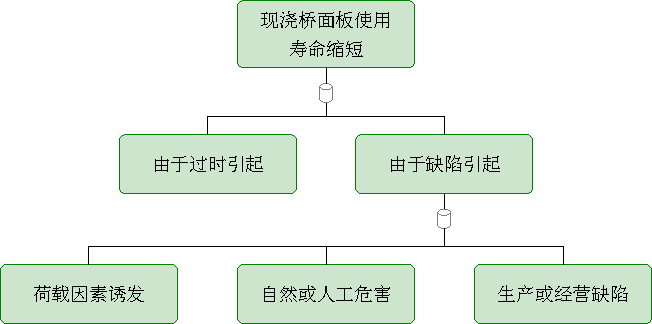
\includegraphics{fault-tree-deck.pdf}
  \caption{桥面系\gls*{faulttree}的起点}\label{fig:fault-tree-deck}
\end{figure}

% In \cref{fig:fault-tree}, either of two main factors is shown to be capable of contributing to reduced service life of a bridge deck: obsolescence or deficiency. The elliptical symbol just above these two factors is referred to as an “or gate,” which signifies that either one of the factors below it could result in reduced service life. The fault tree shown in \cref{fig:fault-tree} continues to list the major categories of factors that could result in reduced service life of bridge deck, those related to induced loads, natural or man-made hazards, and production/operation defects.

在 \cref{fig:fault-tree-deck} 中,两个主要因素中的任何一个都被证明能够导致桥面板的\gls*{servicelife}缩短:过时或缺陷。这两个因素上方的圆柱体符号称为“或门”,表示其下方的任何一个因素都可能导致\gls{servicelife}缩短。 \cref{fig:fault-tree-deck} 中显示的\gls*{faulttree}继续列出可能导致桥面板\gls{servicelife}缩短的主要因素类别,这些因素与感应载荷、自然或人为危害以及生产/运营有关缺陷。

% \cref{fig:fault-tree-deck-con}, shows the continuation of the fault tree for breakdown of factors related to load-induced factors for bridge deck.
\cref{fig:fault-tree-deck-con} 显示了\gls*{faulttree}的延续,用于分解由桥面板的负载引起的相关因素。

\begin{figure}
  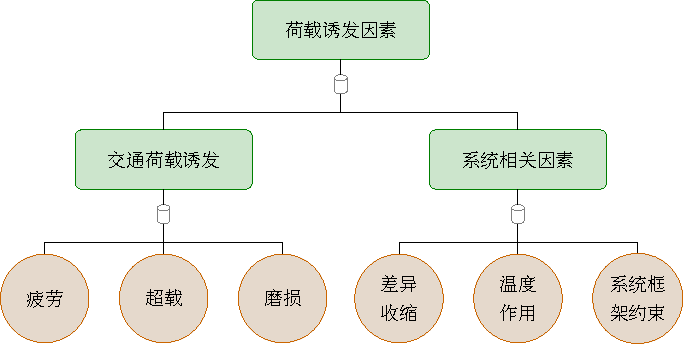
\includegraphics{fault-tree-deck-con.pdf}
  \caption{桥面系\gls*{faulttree}的延续}\label{fig:fault-tree-deck-con}
\end{figure}

% In \cref{fig:fault-tree-deck-con}, the factors related to load-induced are subcategorized into traffic-induced loads or loads induced by system-dependent loads factors, such as restraints provided by shear studs, etc. As shown in \cref{fig:fault-tree-deck-con}, two factors are further broken down into subcomponents, each capable of reducing the service life of bridge deck. The factors inside the circles are the basic factors without any further subcomponent. They represent the end of that branch of the fault tree and require the development of individual strategies to mitigate them. This aspect of process is described later.

在 \cref{fig:fault-tree-deck-con} 中,与荷载相关的因素被细分为交通引起的荷载或由系统相关荷载因素引起的荷载,例如剪力钉提供的约束等。如 \cref{fig:fault-tree-deck-con} 所示,两个因素进一步分解为子组件,每个子组件都会降低桥面板的\gls{servicelife}。圆圈内的因素是没有任何进一步子成分的基本因素。它们代表\gls*{faulttree}分支的末端,需要制定单独的策略来缓解它们。这方面的过程将在后面描述。

% In the Guide, each element of the fault tree is described immediately after introducing each branch of the fault tree. It is advisable to do the same when developing customized fault trees for major and complex bridges. Documentation of factors affecting the service life of bridge elements, components, or subsystems in the form of a fault tree, should be part of the overall plan for design for service life and provided to the owner for future reference.

在\bkn{指南}中,在介绍了\gls*{faulttree}的每个分支后,立即对\gls*{faulttree}的每个元素进行了描述。在为主要和复杂的桥梁开发定制\gls*{faulttree}时,建议这样做。以\gls*{faulttree}的形式记录影响桥梁\gls{element}、\gls{component}或\gls{subsystem}\gls{servicelife}的因素,应作为\gls{servicelife}设计总体计划的一部分,并提供给业主以供将来参考。

% \subsubsection*{Mitigation Strategies}
\subsubsection*{缓解策略}

% Where possible, each chapter provides provable solutions for major factors affecting the service life of a particular bridge element, component, subsystem, or system. Some chapters also include technology tables that summarize major characteristics associated with each solution and provide the potential solutions to factors affecting service life in a form that is easier to comprehend. For example, Figure 1.9 shows the part of the technology tables summarizing solutions for enhancing service life of bridge decks and related to traffic-induced loads as shown in \cref{fig:fault-tree-deck-con}. In \cref{fig:fault-tree-deck-con}, as part of the fault tree for bridge deck, traffic-induced loads is identified as one factor capable of reducing the service. In \cref{fig:fault-tree-deck-con}, below traffic-induced loads, three basic factors capable of reducing the service life of bridge deck are identified: Fatigue, Overload and Wear and Abrasion. Each basic factor needs to be mitigated using a select strategy, and in almost all cases, there is more than one strategy to mitigate these basic factors. It is good practice to collect these strategies in table form and select the optimal strategy, considering its interaction with other parts of bridge. The technology tables provided in various chapters of the Guide summarize strategies that can be used to mitigate various basic factors capable of reducing service life. For major and complex bridges the list of strategies could be different and based on local preferences and experiences. Most agencies have access to field data collected over the years, which could be used to construct customized strategy tables for the purpose of mitigating basic factors capable of reducing service life of bridge elements, components and subsystems.

在可能的情况下,每一章都为影响特定桥梁\gls{element}、\gls{component}、\gls{subsystem}或\gls{system}\gls{servicelife}的主要因素提供了可证明的解决方案。一些章节还包括技术表,这些表总结了与每个解决方案相关的主要特性,并以更容易理解的形式提供了影响\gls{servicelife}的因素的潜在解决方案。例如,\cref{tab:mitigating-factors-deck} 显示了技术表的一部分,总结了提高桥面板\gls{servicelife}的解决方案以及与交通引起的负载相关的解决方案,如 \cref{fig:fault-tree-deck-con} 所示。在 \cref{fig:fault-tree-deck-con} 中,作为桥面板\gls*{faulttree}的一部分,交通引起的负载被确定为能够减少服务的一个因素。在 \cref{fig:fault-tree-deck-con} 中,在交通引起的载荷下,确定了三个能够缩短桥面\gls{servicelife}的基本因素:疲劳、过载和磨损。每个基本因素都需要使用一种选择策略来减轻,并且在几乎所有情况下,都有不止一种策略来减轻这些基本因素。最好以表格形式收集这些策略并选择最佳策略,同时考虑其与桥梁其他部分的交互。本指南各章中提供的技术表总结了可用于减轻各种能够缩短\gls{servicelife}的基本因素的策略。对于主要和复杂的桥梁,策略列表可能会有所不同,并基于当地的偏好和经验。大多数机构都可以访问多年来收集的现场数据,这些数据可用于构建定制的策略表,以减轻能够降低桥梁\gls{element}、\gls{component}和\gls{subsystem}\gls{servicelife}的基本因素。

\begin{table}
  \caption{影响桥面\gls{servicelife}和与交通荷载相关的缓解因素技术表 (Table 4.3)}\label{tab:mitigating-factors-deck}
  \begin{tblr}{
  colspec={c c X[l] X[l] X[l]},
  row{1}={c,bg=genfg,fg=white,font=\bfseries,guard}
}
\SetCell[c=2]{m,c}\glsentrytext{servicelife}问题 & & 缓解策略 & 优点 & 缺点 \\
\SetCell[r=4]{m,c,bg=genbgd!50}{交通\\荷载\\问题} 
& 疲劳                   & 按 \acrshort{lrfd} 规范设计        & 最大限度地减少钢筋失效的可​​能性 & 可能会增加钢材的用量 \\
& 超载                   & 增大桥面板厚度                     & 最大限度地减少开裂             & 增加桥梁结构的重量,增加造价成本 \\
& \SetCell[r=2]{m,c,bg=genbgd!20}磨损 & 调整混凝土配合比设计               & 见 \cref{chp:materials} \nameref{chp:materials} & 见 \cref{chp:materials} \nameref{chp:materials} \\
&                        & 加设薄膜与覆盖层                   & 保护表面不与轮胎直接接触       & 需要每 10 到 20 年进行一次定期维护 \\
\end{tblr}
\end{table}

% The sample table in \cref{tab:mitigating-factors-deck} lists the advantages and disadvantages for each possible solution capable of mitigating the adverse service life consequences of traffic-induced loads. In some cases, more information than just advantages and disadvantages are provided, such as qualitative assessment of maintenance cost. For major and complex bridges additional considerations may be included in technology tables.

\cref{tab:mitigating-factors-deck} 列出了每种可能的解决方案的优缺点,这些解决方案能够减轻交通引起的负载对\gls{servicelife}的不利影响。在某些情况下,提供的信息不仅仅是优点和缺点,例如维护成本的定性评估。对于主要和复杂的桥梁,技术表中可能包含其他考虑因素。

% \subsubsection*{Optimum Selection Strategies}
\subsubsection*{最佳选择策略}
% Overall strategies are provided for achieving enhanced service life. The overall strategy approach provided depends on the particular bridge component, element, subsystem, or system. \cref{fig:overall-strategy} shows an example of the overall strategy for selecting a bearing that meets both strength and service life requirements, taken from \cref{chp:bridge-bearings} of the Guide.

提供的实现延长\gls*{servicelife}的总体策略方法取决于特定的桥梁\gls*{element}、\gls*{component}、\gls*{subsystem}或\gls*{system}。\cref{fig:overall-strategy-bearing} 显示了选择同时满足强度和\gls*{servicelife}要求的支座的总体策略示例,摘自\bkn{指南}的\cref{chp:bridge-bearings}。

\begin{figure}
  % \includegraphics{overall-strategy-bearing.pdf}
  \caption{考虑\gls{servicelife}的支座设计总体策略}\label{fig:overall-strategy-bearing}
\end{figure}

% It should be noted that the chapter devoted to bearings, \cref{chp:bridge-bearings}, identifies factors affecting service life of bearings and provides potential solutions for each. This information, combined with steps outlined in the flowchart, can be used as a rational approach for selecting an appropriate bearing that meets project requirements with emphasis on service life.

应该注意的是,专门介绍支座的章节\cref{chp:bridge-bearings}确定了影响支座\gls{servicelife}的因素,并为每个因素提供了可能的解决方案。此信息与流程图中概述的步骤相结合,可用作选择满足项目要求并强调\gls{servicelife}的合适支座的合理方法。


% \subsubsection*{Examples and Tools}
\subsubsection*{示例与工具}
% Most chapters include examples demonstrating the application of strategies in that chapter.

大多数章节都包含示例以展示该章中策略的应用。

% \section{Quantifying Service Life of Bridge Element, Component, Subsystem, and System}
\section{桥梁\glsentrytext{element}、\glsentrytext{component}、\glsentrytext{subsystem}和\glsentrytext{system}\glsentrytext{servicelife}的量化}

% One of the important steps in developing a systematic, comprehensive service life design plan for bridges is the capability to predict the expected service life of various bridge elements, components, and subsystems, which in turn will dictate the service life of the bridge system. This is Step 9a shown in Figure 1.6. The service life prediction capability is important for developing maintenance, retrofit, and replacement plans, which are an integral part of service life design process. The objective of this section is to provide an overview of the methodology used in the Guide for predicting the service life.
制定系统的、全面的桥梁\gls*{servicelife}设计计划的重要步骤之一是预测各种桥梁\gls*{element}、\gls*{component}和\gls*{subsystem}的预期\gls*{servicelife}的能力,这反过来将决定桥梁系统的\gls*{servicelife}。 这是\cref{fig:general-flowchart}中所示的步骤 9a。 \gls*{servicelife}预测能力对于制定维护、改造和更换计划非常重要,这些都是\gls*{servicelife}设计过程中不可或缺的一部分。 本节的目的是概述\bkn{指南}中用于预测\gls*{servicelife}的方法。

% Bridge elements, components, subsystems, and systems are subject to the effects of traffic and the environment. These external sources of deterioration act through various mechanisms to cause actual deterioration of bridge elements and eventually failure. The mechanisms of deterioration are the physical laws that govern such deterioration. Deterioration rates can be described using mathematical expressions or empirical/semiempirical models, which are developed using data collected by field monitoring of bridges, laboratory generated data, expert opinions, or combination of available data. Service life is also affected by risk to damage either from traffic or extreme environmental occurrences. The acceptability of this damage is evaluated based on risk. Service life can be extended by minimizing risk or designing for appropriate levels of extreme occurrences.
桥梁\gls*{element}、\gls*{component}、\gls*{subsystem}和\gls*{system}会受到交通和环境的影响。 这些外部\gls*{deterioration}源通过各种机制起作用,导致桥梁\gls{element}实际\gls*{deterioration}并最终失效。 \gls*{deterioration}机制是支配这种\gls*{deterioration}的物理定律。 可以使用数学表达式或经验/半经验模型来描述\gls*{deterioration}率,这些模型是使用桥梁现场监测收集的数据、实验室生成的数据、专家意见或可用数据的组合开发的。 \gls*{servicelife}还受到交通或极端环境事件造成的损坏风险的影响。 这种损害的可接受性是根据风险来评估的。 通过最大限度地降低风险或针对极端事件的适当级别进行设计,可以延长\gls*{servicelife}。

% Enhanced service life for bridge elements, components, subsystems, and systems can be achieved through:
可以通过以下方式延长桥梁\gls*{element}、\gls*{component}、\gls*{subsystem}和\gls*{system}的\gls*{servicelife}:

\begin{itemize}
  % \item Use of durable materials,
  \item 使用耐久性材料;
  % \item Use of either passive or active protection systems,
  \item 使用主动或被动的保护系统;
  % \item Optimum selection of details,
  \item 采用最佳细部构造;
  % \item Optimum maintenance and repair,
  \item 采用最佳的运营维护和维修;
  % \item Reduced service level,
  \item 降低服务水平;
  % \item Increased factor of safety or reduction in stress levels, and
  \item 增加安全系数或降低应力水平;
  % \item Isolation from risk damage.
  \item 隔离风险损害。
\end{itemize}

% To estimate the service life of bridge elements, components, or subsystems quantitatively, the following information is needed:
要定量估算桥梁\gls*{element}、\gls*{component}或\gls*{subsystem}的\gls*{servicelife},需要以下信息:
\begin{itemize}
  % \item Source of deterioration,
  \item \gls*{deterioration}产生的根源;
  % \item Deterioration mechanism,
  \item \gls*{deterioration}机制;
  % \item Deterioration models, and
  \item \gls*{deterioration}模型;
  % \item Failure modes.
  \item 失效模式。
\end{itemize}

% The following sections provide information on each of these items.
以下部分提供了有关其中每一项的信息。

\subsubsection*{\gls*{deterioration}产生的根源}
% Traffic related or environmental effects form the basic external cause of deterioration. For example, deicing compounds, an external source of deterioration, can result in corrosion of reinforcement in bridge elements
交通相关或环境影响构成\gls*{deterioration}的基本外部原因。例如,除冰化合物是\gls*{deterioration}的外部来源,会导致桥梁\gls{element}中钢筋的腐蚀。

\subsubsection*{\gls*{deterioration}机制}
% Deterioration is governed by a process called the deterioration mechanism. For example, sliding surfaces in bearings experience deterioration through horizontal movement and friction between sliding materials, created by truck passages or temperature fluctuations. The horizontal movement and friction in this instance is the deterioration mechanism. In the case of concrete elements, ingress of chloride through concrete causes initiation of corrosion in unprotected steel reinforcement. In this instance, the ingress of chloride is the deterioration mechanism.
控制\gls*{deterioration}的过程的机理称之为\gls*{deterioration}机制。例如,支座的滑动表面会因卡车通行或温度波动造成的水平运动和滑动材料之间的摩擦而\gls*{deterioration}。 这种情况下的水平运动和摩擦是\gls*{deterioration}机制。 对于混凝土构件,氯离子渗透通过混凝土会导致未受保护的钢筋发生腐蚀。 在这种情况下,氯离子的渗透是\gls*{deterioration}机制。

\subsubsection*{\gls*{deterioration}模型}
% Deterioration models are used to describe the rate of deterioration. They describe the relationship between the condition of the bridge (or its element) and its time of use, and show how the bridge deteriorates over time. It assumes that no replacements or major repairs are made, but it usually implies that scheduled maintenance actions are performed as planned. The basic model applies either to a bridge system as a whole, or to any of its subsystems, components or elements.
\gls*{deterioration}模型用于描述\gls*{deterioration}率。 它们描述了桥梁(或其\gls*{element})的状况与其使用时间之间的关系,并显示了桥梁如何随着时间的推移而\gls*{deterioration}。 它假设没有进行任何更换或大修,但通常意味着按计划执行了定期维护操作。 基本模型既适用于整个桥梁\gls*{system},也适用于其任何\gls*{subsystem}、\gls*{component}或\gls*{element}。

% An example of a deterioration curve is presented in \cref{fig:bridge-deterioration-curve}. If the bridge is placed in service at period T0, its condition gradually declines, and the deterioration curve represents its condition over time. Initially the condition is good, but after a period of wear and aging, it eventually (at time Tf) reaches an unacceptably low condition Cf. The time period between T0 and Tf is called Service Life (SL) of the bridge.
\cref{fig:bridge-deterioration-curve} 中给出了\gls*{deterioration}曲线的一个例子。 如果桥梁在 $T_0$ 期间投入使用,其状况会逐渐下降,\gls*{deterioration}曲线表示其随时间变化的状况。最初状况良好,但经过一段时间的磨损和老化后,最终(在时间 $T_\text{f}$)达到无法接受的低状况 $C_\text{f}$。 $T_0$ 和 $T_\text{f}$ 之间的时间段称为桥梁的\acrfull{sl}。

\begin{figure}
  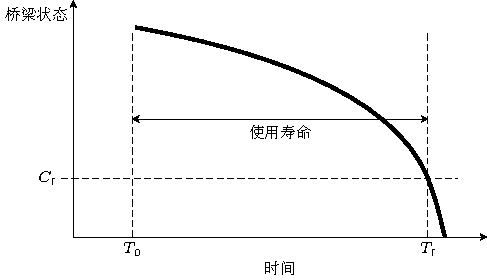
\includegraphics{bridge-deterioration-curve.pdf}
  \caption{桥梁\gls*{deterioration}曲线示例}\label{fig:bridge-deterioration-curve}
\end{figure}

% In practice, the development of realistic behavioral deterioration models is a data-intensive process complicated by lack of knowledge of the underlying physical and chemical processes fostering deterioration, as well as by the data availability. At the present time the available deterioration models, which are based on long-term data collection, are very limited. Further, as time passes, the quality of the bridge design and construction improves. As a result, application of data collected from existing bridges to predict performance of future bridges should be practiced with caution.
在实践中,现实行为\gls*{deterioration}模型的开发是一个数据密集型过程,由于缺乏对促进\gls*{deterioration}的潜在物理化学过程的知识以及数据可用性而变得复杂。目前,基于长期数据收集的可用\gls*{deterioration}模型非常有限。此外,随着时间的推移,桥梁设计和施工的质量也会提高。因此,应谨慎应用从现有桥梁收集的数据来预测未来桥梁的性能。

% Deterioration models capable of quantitatively predicting the service life of bridge elements, components, subsystems, or systems are very limited or nonexistent. The most acceptable deterioration model is in the form of the solution to Fick's second law, used to predict the rate of chloride ingress through concrete cover. This model, including its limitations, is described in \cref{chp:corrosion-of-steel-rc-bridge} of the Guide. It is expected that with time, more deterioration models will become available and will greatly enhance quantification of the service life of bridge elements, components, subsystems, or systems.
能够定量预测桥梁\gls*{element}、\gls*{component}、\gls*{subsystem}或\gls*{system}\gls*{servicelife}的\gls*{deterioration}模型非常有限或不存在。最可接受的\gls*{deterioration}模型采用菲克第二定律的解形式,用于预测氯离子通过混凝土保护层的侵入率。该模型及其局限性在\bkn{指南}的 \cref{chp:corrosion-of-steel-rc-bridge} 中进行了描述。预计随着时间的推移,将有更多的\gls*{deterioration}模型可用,并将大大提高桥梁\gls*{element}、\gls*{component}、\gls*{subsystem}或\gls*{system}\gls*{servicelife}的量化。

% As shown on \cref{fig:condition-life-cycle}, if left alone a bridge will deteriorate over the period of its service life. However, in most cases a bridge is not left to follow the basic deterioration path and reach an unacceptable condition without interruption. The agency responsible for the bridge will from time to time undertake repairs, rehabilitations, and renewals that return conditions to higher levels and extend its service life. During these interventions, the condition rate of the bridge condition increases, as depicted in \cref{fig:condition-life-cycle}.
如\cref{fig:condition-life-cycle} 所示,如果任其发展,桥梁状况将在其\gls*{servicelife}期间\gls*{deterioration}。然而,在大多数情况下,桥梁不会沿着基本的\gls*{deterioration}路径发展并在不中断的情况下达到不可接受的状态。桥梁主管机构将不时进行维修、修复和更新,使桥梁状况恢复到更高水平并延长其\gls*{servicelife}。在这些干预期间,桥梁状况的状况率增加,如\cref{fig:condition-life-cycle} 中所示。

\begin{figure}
  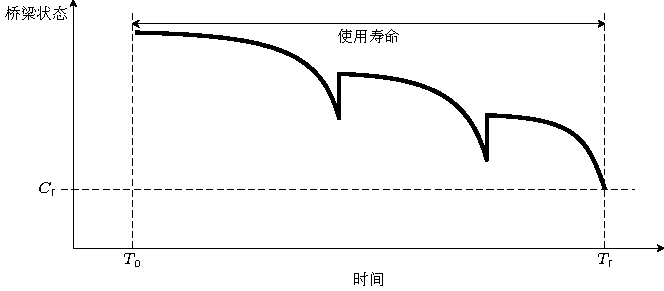
\includegraphics{condition-life-cycle.pdf}
  \caption{桥梁在整个生命周期内状况}\label{fig:condition-life-cycle}
\end{figure}

% Deterioration models can also be based on some level of understanding of the mechanism governing the deterioration and the capability to express the process using a mathematical expression. An example is deterioration of concrete elements because of chloride induced corrosion of reinforcement. The assumption is that ingress of chloride through the concrete element is governed by Fick's second law, which assumes a homogeneous material.

\gls*{deterioration}模型可以基于对控制\gls*{deterioration}机制的某种程度的理解以及运用数学表达式表达其过程的能力。一个例子是由于氯离子引起的钢筋腐蚀而导致混凝土构件\gls*{deterioration}。这其中,我们假定混凝土材料是均质的,氯离子在混凝土中的渗透符合菲克第二定律。

% In the case of chloride and carbonation induced corrosion, there is some level of agreement within the scientific community as to the existence of deterioration models. However, for other deterioration modes such as sulfate attack, alkali-silica reactivity (ASR), and freeze/thaw or wear and abrasion, there is a lack of adequate models. Further, as described earlier, the use of deterioration models to predict the time to initiate corrosion of reinforcement embedded within certain distances of the concrete surface because of chloride ingress, should be approached with caution. Following is brief description of a deterioration model for chloride induced corrosion.

在氯离子和碳化引起的腐蚀的情况下,科学界对\gls*{deterioration}模型存在一定程度的共识。然而,对于其他\gls*{deterioration}模式,如硫酸盐侵蚀、\acrlong{asr}(\acrshort{asr})、冻融或磨损,缺乏足够的模型。此外,如前所述,使用\gls*{deterioration}模型来预测由于氯离子渗透混凝土表面一定距离内的钢筋开始腐蚀的时间,应谨慎处理。以下是氯离子引起的腐蚀的\gls*{deterioration}模型的简要描述。

% There are different approaches to solving Fick's second law. A finite difference approach, or the use of error functions, is reported in published literatures. Equation 1.4 is an error function solution of Fick's second law, capable of predicting the chloride concentration level at various depths within the concrete element.

求解菲克第二定律有不同的方法。已发表的文献采用了有限差分法或误差函数解法。\cref{eq:ficks-second-law} 是菲克第二定律的误差函数解,能够预测混凝土构件内不同深度的氯离子浓度水平。
\begin{equation}
  \label{eq:ficks-second-law}
  C_\text{crit} = C(x=a, t) = C_0 +(C_{\text{S},\Delta x} - C_0)\left[ 1-\erf 
   \frac{a-\Delta x}{2\sqrt{D_{\text{app},\text{C}}\cdot t}} \right]
\end{equation}
\begin{EqDesc}{C(x,t)}
  \item[C_\text{crit}] 临界氯离子含量(重量百分比 \%);
  \item[C(x,t)] 在深度 $x$(结构表面:$x=\qty{0}{mm}$)处和时间 $t$ 时混凝土中氯离子的含量(重量百分比 \%);
  \item[C_0] 混凝土初始氯离子含量(重量百分比 \%);
  \item[C_{\text{S},\Delta x}] 深度 $\Delta x$ 处和某个时间点 $t$ 的氯离子含量(重量百分比 \%);
  \item[x] 对应氯离子含量 $C(x,t)$ 的深度(\unit{mm});
  \item[a] 混凝土保护层(\unit{mm});
  \item[\Delta x]对流区(混凝土中氯离子渗透过程不同于菲克第二扩散定律的部分)深度(\unit{mm});
  \item[D_{\text{app},\text{C}}] 氯离子在混凝土中的表观扩散系数(\unit{mm^2/yr});
  \item[t] 时间(\unit{yr});
  \item[\erf] 误差函数。
\end{EqDesc}

% \cref{eq:ficks-second-law} should be used in conjunction with probabilistic approaches to account for variability of several parameters, such as apparent coefficient of diffusion, chloride concentration, and critical chloride level to start corrosion. Furthermore, the diffusivity of concrete through different layers of concrete element is not uniform. \cref{eq:ficks-second-law} predicts the chloride content in the structure at a given depth (x) and time (t). This number is given by the left-hand side of the equation, C(x,t).

\cref{eq:ficks-second-law} 应与概率方法结合使用,以解释多个参数的可变性,例如表观扩散系数、氯离子浓度和开始腐蚀的临界氯离子水平。此外,混凝土通过不同层的混凝土的扩散率是不均匀的。 \cref{eq:ficks-second-law} 预测给定深度($x$)和时间($t$)下结构中的氯离子含量。该数字由等式的左侧 $C(x,t)$ 给出。

% The C(x,t) obtained from \cref{eq:ficks-second-law} is then compared to the critical chloride content, Ccrit , which is the value determined to be the point at which corrosion starts. When the chloride level at a given depth, x, of the structure is reached, the critical value, the corrosion is assumed to initiate. The service life of concrete element can then be assumed to consist of the time period to initiate corrosion plus the time period for propagation of the corrosion to the point that will limit the functionality of concrete element. This process is depicted in \cref{fig:damage-service-life}.

将从\cref{eq:ficks-second-law} 获得的 $C(x,t)$ 与临界氯离子含量 $C_\text{crit}$ 进行比较,该值被确定为腐蚀开始点。当结构的给定深度 $x$ 处的氯离子水平达到临界值时,我们认为腐蚀开始。然后可以假定混凝土的\gls{servicelife}包括开始腐蚀的时间段加上腐蚀传播到将限制混凝土功能的点的时间段。这个过程在\cref{fig:damage-service-life} 中描述。

\begin{figure}
  % \includegraphics[width=\linewidth]{graphic-file}
  % \caption{Relationship between damage and service life. (Source COWI, Denmark)}
  \caption{损伤与\gls*{servicelife}的关系}
  \label{fig:damage-service-life}
\end{figure}

\subsubsection*{失效模式}
% Sources of deterioration (such as deicing compounds), acting through deterioration mechanisms (such as ingress of chloride through concrete cover), and described by deterioration models (such as solution to Fick's second law) result in failure modes (corrosion of reinforcement, causing corrosion induced cracking and loss of strength). The final failure could consist of several stages, such as start and propagation phases.
\gls*{deterioration}源(例如除冰盐等化合物)通过\gls*{deterioration}机制(例如氯离子渗透通过混凝土保护层)起作用,并由\gls*{deterioration}模型(如菲克第二定律的解)描述导致失效模式(钢筋腐蚀,导致腐蚀引起开裂和强度损失)。最终故障可能包括几个阶段,例如开始阶段和传播阶段。

\subsubsection*{\glsentrytext{servicelife}评估}
% In the Guide, two general philosophies are presented to estimate the service life of bridge elements, components, and subsystems. The end result of quantifying the service life of bridge elements, components, or subsystems is to establish the ts, the service life of bridge elements, components, or subsystems, and compare it to specified service life of the bridge system to determine the need for retrofit or replacement strategies if needed.
\bkn{指南}提出了两种一般性原理来估算桥梁\gls*{element}、\gls*{component}和\gls*{subsystem}的\gls*{servicelife}。量化桥梁\gls*{element}、\gls*{component}或\gls*{subsystem}\gls*{servicelife}的最终结果是建立桥梁\gls*{element}、\gls*{component}或\gls*{subsystem}的\gls*{servicelife} $t_\text{s}$,并将其与桥梁\gls*{system}的指定\gls*{servicelife}进行比较以确定是否需要改造或更换策略。

% Two general design approaches for service life are:
两种通用的\gls*{servicelife}设计方法是:
\begin{itemize}
  \item 有限\gls*{servicelife}法;
  \item 目标\gls*{servicelife}法。
\end{itemize}

% When the design service life, ts, of the bridge element, component, or subsystem, established through one of the two design approaches for service life philosophies is less than the specified design life of the bridge system, tD, the bridge element, component, or subsystem under consideration could be replaced to achieve the specified design life of the bridge system.
当通过两种\gls*{servicelife}理念设计方法之一确定的桥梁\gls*{element}、\gls*{component}或\gls*{subsystem}的设计\gls*{servicelife} $t_\text{s}$ 小于桥梁\gls*{system}的指定\gls*{designlife} $t_\text{D}$ 时,桥梁\gls*{element}、\gls*{component}、 或正在考虑的\gls*{subsystem}可以更换,以达到桥梁\gls*{system}的指定\gls*{designlife}。

% The major difference between the two approaches for service life design is the existence of well-accepted deterioration models, which is needed before using the finite service life approach.
两种\gls*{servicelife}设计方法的主要区别在于存在广为接受的\gls*{deterioration}模型,这是在使用有限\gls*{servicelife}方法之前所必需的。

\paragraph*{有限\gls*{servicelife}法}
% Bridge elements, components, and subsystems designed using the finite service life approach, should have service life that is greater than or equal to specified bridge system service life. Otherwise, the bridge element, component, or subsystem under consideration must be retrofitted or replaced to allow the bridge to continue providing its intended function until reaching the specified bridge system service life. In the finite service life approach, the service life of the bridge components, elements, or subsystems is estimated using well-accepted deterioration models. The existence of deterioration models is therefore essential for use of the finite service life approach.
使用有限\gls*{servicelife}方法设计的桥梁\gls*{element}、\gls*{component}和子系统的\gls*{servicelife}应大于或等于指定的桥梁\gls*{system}\gls*{servicelife}。 否则,必须对所考虑的桥梁\gls*{element}、\gls*{component}或\gls*{subsystem}进行改造或更换,以使桥梁继续提供其预期功能,直至达到规定的桥梁\gls*{system}\gls*{servicelife}。 在有限\gls*{servicelife}法中,桥梁\gls*{component}、\gls*{element}或\gls*{subsystem}的\gls*{servicelife}使用广为接受的\gls*{deterioration}模型进行估算。 因此,\gls*{deterioration}模型的存在对于使用有限\gls*{servicelife}方法是必不可少的。

% The deterioration models are generally developed using one of the following approaches:
\gls*{deterioration}模型通常使用以下方法之一开发:
% \begin{itemize}
%   \item Mathematical models which describe the deterioration rate. These models could be approximate or based on laws of physics.
%   \item Empirical or semiempirical models developed using data collected from laboratory or field performance of bridges. Fatigue models used in the LRFD Specifications is an example of empirical deterioration model.
%   \item Empirical models based on expert opinions or experiences. Examples include various models used in \pontis.
% \end{itemize}
\begin{itemize}
  \item 描述\gls*{deterioration}率的数学模型。这些模型可以基于物理定律或是近似的。
  \item 使用从实验室或桥梁现场性能收集的数据开发的经验或半经验模型。 例如 \lrfd 中使用的疲劳模型即是一个经验\gls*{deterioration}模型。
  \item 基于专家意见或经验的经验模型。 例如 \pontis 中使用的各种模型。
\end{itemize}

% Where deterioration models exist, the service life design could be in the form of:
在存在\gls*{deterioration}模型的情况下,使用寿命设计可以采用以下形式:

% \emph{Full probabilistic approach}. This approach requires having probability distribution functions for all variables used in the deterioration model.
\emph{全概率方法}。这种方法需要为恶化模型中使用的所有变量提供概率分布函数。

% \emph{Semiprobabilistic or partial load factor approach}. This approach is developed using full probabilistic approach. It is equivalent to using load and resistance factors in the LRFD Specifications versus using full probabilistic approach (such as using Mont Carlo simulation) to design or rate bridges.
\emph{半概率或部分荷载系数方法}。 这种方法是使用全概率方法开发的。 它相当于使用 \lrfd 中的荷载—抗力系数与使用完全概率方法(例如使用蒙特卡洛模拟)来设计或评估桥梁。

\paragraph*{目标\gls*{servicelife}法}
% In many instances the deterioration models are not available or their applicability is questionable. In these situations, available alternatives are 
在许多情况下,\gls*{deterioration}模型不可用或它们的适用性值得怀疑。在这些情况下,可用的替代方案是
\begin{enumerate*}
  % \item  use of high performing material that does not deteriorate, such as use of stainless steel, an approach is generally referred to as the avoidance of deterioration method within European practice, or 
  \item 使用不会\gls*{deterioration}的高性能材料,例如使用不锈钢,这种方法在欧洲实践中通常被称为避免\gls*{deterioration}方法;
  % \item use material that based on experience, or based on expert opinion, could provide a specified or a target service life. If the estimated service life of the bridge element, component, or subsystem is less than the specified service life of the bridge, retrofit or replacement strategies must be specified, allowing the bridge system to continue providing its intended function.
  \item 使用基于经验或专家意见的材料,可以提供指定或目标\gls*{servicelife}。如果桥梁\gls*{element}、\gls*{component}或\gls*{subsystem}的估计\gls*{servicelife}小于桥梁的指定\gls*{servicelife},则必须指定改造或更换策略,使桥梁\gls*{system}继续提供其预期功能。
\end{enumerate*}

% The major difference between finite service life and target service life design approaches is that in finite service life design approach, the condition of the bridge element, component, and subsystem can be traced over time using deterioration models, whereas in target service life design approach, only the total expected service life is estimated. The specified target service life of bridge element, component, or subsystem is mainly established based on experience or expert opinion, and could vary significantly from assumed values. Nevertheless, specifying a target service life for a given bridge element, component, or subsystem allows the bridge owner to plan and anticipate necessary maintenance actions and places demands on the designer to incorporate necessary design features where needed. For example, the service life of PTFE sliding surfaces in bearing devices could be assumed to be about ten years (target service life of 10 years). The designer must then incorporate necessary mechanisms to lift the bridge and replace the sliding surfaces, preferably while maintaining traffic. On the other hand, the bridge owner must plan and anticipate the replacement of sliding surfaces every 10 years.
有限\gls*{servicelife}法和目标\gls*{servicelife}法之间的主要区别在于,在有限\gls*{servicelife}法中,可以使用\gls*{deterioration}模型跟踪桥梁\gls*{element}、\gls*{component}和\gls*{subsystem}随时间推移的状况,而在目标\gls*{servicelife}设计方法中,仅估算总预期\gls*{servicelife}。桥梁\gls*{element}、\gls*{component}或\gls*{subsystem}的指定目标\gls*{servicelife}主要是根据经验或专家意见确定的,可能与假定值有很大差异。然而,为给定的桥梁\gls*{element}、\gls*{component}或\gls*{subsystem}指定目标\gls*{servicelife}允许桥梁所有者计划和预测必要的维护行动,并要求设计师在需要时纳入必要的设计特征。例如,支座装置中 \acrlong{ptfe} 滑动表面的\gls*{servicelife}可以假设为大约 10 年(目标\gls*{servicelife}为 10 年)。然后,设计师必须结合必要的机制来提升桥梁并更换滑动表面,最好是在维持交通的同时。另一方面,桥梁所有者必须计划和预期每 10 年更换一次滑动面。

% \section{Owner's Manual}
\section{使用手册}

% In instances where specified by the owner and for major and complex bridges, the final step in the design for service life process is the development of a bridge Owner's Manual, which summarizes the processes used for design for service life and provides complete descriptions of outcomes and recommendations. The intention is to equip the owner with the necessary knowledge to keep the bridge operational for the specified service life period. The bridge Owner's Manual should be provided to the owner at the time of opening the bridge to traffic, following an independent review process described in the next section.

在业主指定的情况下,对于主要的和复杂的桥梁,\gls{servicelife}设计流程的最后一步是制定桥梁使用手册,该手册总结了\gls{servicelife}设计所使用的流程,并提供了对结果的完整描述和建议。目的是让业主掌握必要的知识,使桥梁在指定的\gls{servicelife}期间保持正常运行。桥梁使用手册应在桥梁通车时提供给业主,并遵循下一节所述的独立审查程序。

% The entire process used for design for service life should be well documented and include assumptions, limitations, and any other information of which the owner should be aware, including complete information with respect to “hot spots” within various bridge elements, components, or subsystems that will require closer inspection, maintenance, retrofit, or replacement. The Owner's Manual should include a complete management plan with respect to service life, including information on timely maintenance actions, and identify replacement items and methodologies for replacement with information on the required level of traffic interruption, if any. In the case of major and complex bridges it is suggested that a bridge instrumentation and monitoring plan be developed and be tied to the bridge service life management plan. Additional information to be included in the Owner's Manual after construction should include the actual material properties of critical bridge elements versus the assumed values used in the design process. Such information is important for future bridge rating.

用于\gls{servicelife}设计的整个过程应妥善记录,这其中包括假定、限制和所有者应了解的任何其他信息,如需要更仔细的检查、维护、改造或更换的有关各种桥梁\gls{element}、\gls{component}或\gls{subsystem}中“热点”的完整信息。用户手册应包括有关\gls{servicelife}的完整管理计划,包括有关及时维护措施的信息,确定更换项目和更换方法以及所需交通中断级别的信息(如果有)。对于大型和复杂的桥梁,建议制定桥梁检测和监测计划,并将其与桥梁\gls{servicelife}管理计划联系起来。施工后要包含在用户手册中的其他信息应包括关键桥梁\gls{element}的实际材料特性与设计过程中使用的假定值的对比。这些信息对未来的桥梁评级很重要。

% With respect to major and complex bridges, the designer should use sound engineering judgment for determining the level and extent of information to be included in the Owner's Manual. The bridge Owner's Manual is analogous to the design calculations that are customarily provided to the bridge owner, except that the Owner's Manual contains much more detailed information.

对于主要和复杂的桥梁,设计者应使用合理的工程判断来确定要包含在用户手册中的信息的级别和范围。桥梁所有者手册类似于通常提供给业主的设计计算,只是所有者手册包含更多详细信息。

% \section{Independent Review of Design for Service Life Process}
\section{\glsentrytext{servicelife}设计过程的独立审查}

% The design for service life processes, results, and recommendations as summarized in the bridge Owner's Manual, should be checked by an independent and knowledgeable third party. This independent check is analogous to an independent design check typically conducted for bridge design.

桥梁用户手册中总结的\gls{servicelife}设计的过程、结果和建议应由独立且有经验的第三方进行检查。这种独立检查类似于通常针对桥梁设计进行的独立设计检查。

% \section{Summary of Steps for Design for Service Life for Specific Bridge Element, Component, and Subsystem}\label{sec:summary-steps}
\section{特定桥梁\glsentrytext{element}、\glsentrytext{component}和\glsentrytext{system}的\glsentrytext{servicelife}设计步骤总结}\label{sec:summary-steps}

% This section provides a summary of the steps in design for service life. Detailed description of individual steps is provided in \cref{sec:guide-approach}.

本节总结了\gls{servicelife}设计的步骤。 \cref{sec:guide-approach} 中提供了各个步骤的详细说明。

% Bridge elements, components, and subsystems can deteriorate at different rates and have different service lives. This governs the service life of a bridge system, which is reached when the service life of critical bridge elements, components, or subsystems is exhausted beyond being repaired or replaced economically or because of other considerations.

桥梁\gls{element}、\gls{component}和\gls{subsystem}可能会以不同的速度\gls*{deterioration}并具有不同的\gls{servicelife}。这决定了桥梁\gls{system}的\gls{servicelife},当关键桥梁\gls{element}、\gls{component}或\gls{subsystem}的\gls{servicelife}耗尽而无法经济地修复或更换或出于其他考虑时,就会达到桥梁\gls{system}的\gls{servicelife}。

% The general steps in design for service life for particular a bridge element, component or subsystem can be summarized are as follows:
特定桥梁\gls{element}、\gls{component}或\gls{subsystem}的\gls{servicelife}设计的一般步骤可概括如下:

\begin{description}[style=nextline,leftmargin=6.5em]
  % \item [步骤 1] Identify the project requirements, particularly those that will influence the service life.
  \item [步骤 1] 确定项目要求,尤其是那些会影响\gls{servicelife}的要求。
  % \item [步骤 2] Identify feasible bridge systems capable of meeting the project demand.
  \item [步骤 2] 确定能够满足项目需求的可行桥梁\gls{system}。
  % \item [步骤 3] Select each feasible bridge system one at a time and complete Steps 4 through 10.
  \item [步骤 3] 一次选择每个可行的桥梁\gls{system}并完成步骤 4 到 10。
  % \item [步骤 4] Identify the factors that influence the service life of bridge elements, components, and subsystems, such as traffic and environmental factors.
  \item [步骤 4] 确定影响桥梁\gls{element}、\gls{component}和\gls{subsystem}\gls{servicelife}的因素,例如交通和环境因素。
  % \item [步骤 5] Identify modes of failures and consequences. For instance, the corrosion of reinforcement causing corrosion induced cracking and loss of strength.
  \item [步骤 5] 确定故障模式和后果。例如,钢筋的腐蚀导致腐蚀导致开裂和强度损失。
  % \item [步骤 6] Identify suitable approaches for mitigating the failure modes or assessing risk of damage, through life cycle cost analysis. For example, use of better performing materials for sliding surfaces in bearings or use of material prone to deterioration at lower initial cost.
  \item [步骤 6] 通过\acrlong{lcca},确定减轻故障模式或评估损坏风险的合适方法。例如,在支座的滑动表面使用性能更好的材料,或者以较低的初始成本使用易于\gls*{deterioration}的材料。
  % \item [步骤 7] Modify the bridge element, component, or subsystem under consideration, using the selected strategy and ensure compatibility of different strategies used for various bridge elements, components, or subsystems. This step may involve the need to develop several alternatives.
  \item [步骤 7] 使用选定的策略修改考虑中的桥梁\gls{element}、\gls{component}或\gls{subsystem},并确保用于各种桥梁\gls{element}、\gls{component}或\gls{subsystem}的不同策略的兼容性。此步骤可能需要开发多种替代方案。
  % \item [步骤 8] For each modified alternative, estimate the service life of the bridge element, component or subsystem using Finite or Target Service Life Design approaches.
  \item [步骤 8] 对于每个修改后的备选方案,使用有限或目标\gls{servicelife}设计方法估算桥梁\gls{element}、\gls{component}或\gls{subsystem}的\gls{servicelife}。
  % \item [步骤 9] For each modified alternative, compare the service life of the bridge element, component, or subsystem to the service life of the bridge system and develop appropriate maintenance, retrofit, and/or replacement plan.
  \item [步骤 9] 对于每个修改后的备选方案,将桥梁\gls{element}、\gls{component}或\gls{subsystem}的\gls{servicelife}与桥梁\gls{system}的\gls{servicelife}进行比较,并制定适当的维护、改造和/或更换计划。
  % \item [步骤 10] For each modified alternative, develop design, fabrication, construction, operation, maintenance, replacement, and management plans for achieving the specified design life for the bridge system.
  \item [步骤 10] 对于每个修改后的备选方案,制定设计、制造、施工、运营、维护、更换和管理计划,以实现桥梁\gls{system}的指定设计寿命。
  % \item [步骤 11] For each modified alternative, conduct life cycle cost analysis for each feasible bridge system meeting strength and service life requirements, and select the optimum bridge system
  \item [步骤 11] 对于每个修改方案,对每个满足强度和\gls{servicelife}要求的可行桥梁\gls{system}进行生命周期成本分析,选择最佳桥梁\gls{system}
  % \item [步骤 12] When specified by the owner or in cases of major and complex bridges, document the entire design for service life processes in a document called the Owner's Manual. Conduct an independent review of the document and provide it to bridge owner at the time of opening the bridge to traffic.
  \item [步骤 12] 当业主指定或在大型和复杂桥梁的情况下,在称为业主手册的文件中记录\gls{servicelife}过程的整个设计。对文件进行独立审查,并在桥梁通车时将其提供给桥梁所有者。
\end{description}

% \section{Approaches to Using the Guide}
\section{《指南》的使用方法}
% This section provides a limited example demonstrating the use of the Guide and how to implement systematic approaches for design for service life. The example is not inclusive and considers an isolated component of the bridge without considering the remaining bridge elements, components, or subsystems. Further, the example, for the sake of demonstration, uses Life-365, which has limitations when applied to horizontal surfaces, such as bridge decks. Life-365 uses the solution to Fick's second law to predict deterioration of concrete elements subjected to chloride ingress. While this approach has merits for vertical surfaces, such as columns under compression, its applicability to horizontal surfaces, such as bridge deck, is not warranted. In the case of bridge decks, the existence of cracks violates the assumption of a homogeneous material in Fick's second law. The use of Life-365 for the bridge deck example here is for demonstration purposes, as it includes life cycle cost analysis in addition to predicting time to initiate corrosion and propagation.

本节提供了一个有限的示例,演示了\bkn{指南}的使用以及如何实施系统的\gls*{servicelife}设计方法。该示例不是面面俱到的,只考虑了桥梁的一个孤立\gls*{component},而不考虑其余的桥梁\gls*{element}、\gls*{component}或\gls*{subsystem}。此外,为了演示,该示例使用了 \gls{life365},它在应用于水平表面(例如桥面)时具有局限性。\gls{life365} 使用菲克第二定律的解决方案来预测受氯离子渗透影响的混凝土构件的\gls*{deterioration}。虽然这种方法对垂直表面(例如受压柱)有好处,但不能保证它对水平表面(例如桥面板)的适用性。在桥面板的情况下,裂缝的存在违反了菲克第二定律中均质材料的假设。此处将 \gls{life365} 用于桥面示例仅用于演示目的,因为除了预测开始腐蚀和传播的时间之外,它还包括生命周期成本分析。

% The following sections provide an overall description of the bridge used for the example, and illustrate the steps taken in design for service life for one component of the bridge in isolation.
以下各节对示例中使用的桥梁进行了全面描述,并单独说明了桥梁某一\gls{component}的\gls{servicelife}设计所采取的步骤。

% \subsection{Example Bridge Description}
\subsection{桥梁描述示例}
% The example bridge is a 1400-ft long structure carrying four lanes of high volume traffic with pedestrian sidewalks and bicycle lanes. The bridge crosses over low-volume urban local roads, a railroad, and a navigable waterway. Refer to \cref{fig:bridge-aerial,fig:typical-section} for a rendering of the project concept. \cref{fig:superstructure-section} shows the bridge deck system that will be used for this example.

示例桥梁是一座长约 \qty{430}{m} 的结构,承载四条车道,交通繁忙,设有人行道和自行车道。桥梁横跨低流量的城市地方道路、铁路和航道。有关项目的概念性鸟瞰,请参阅\cref{fig:bridge-aerial,fig:typical-section}。 \cref{fig:superstructure-section} 显示了将用于此示例的桥面系。

\begin{figure}
  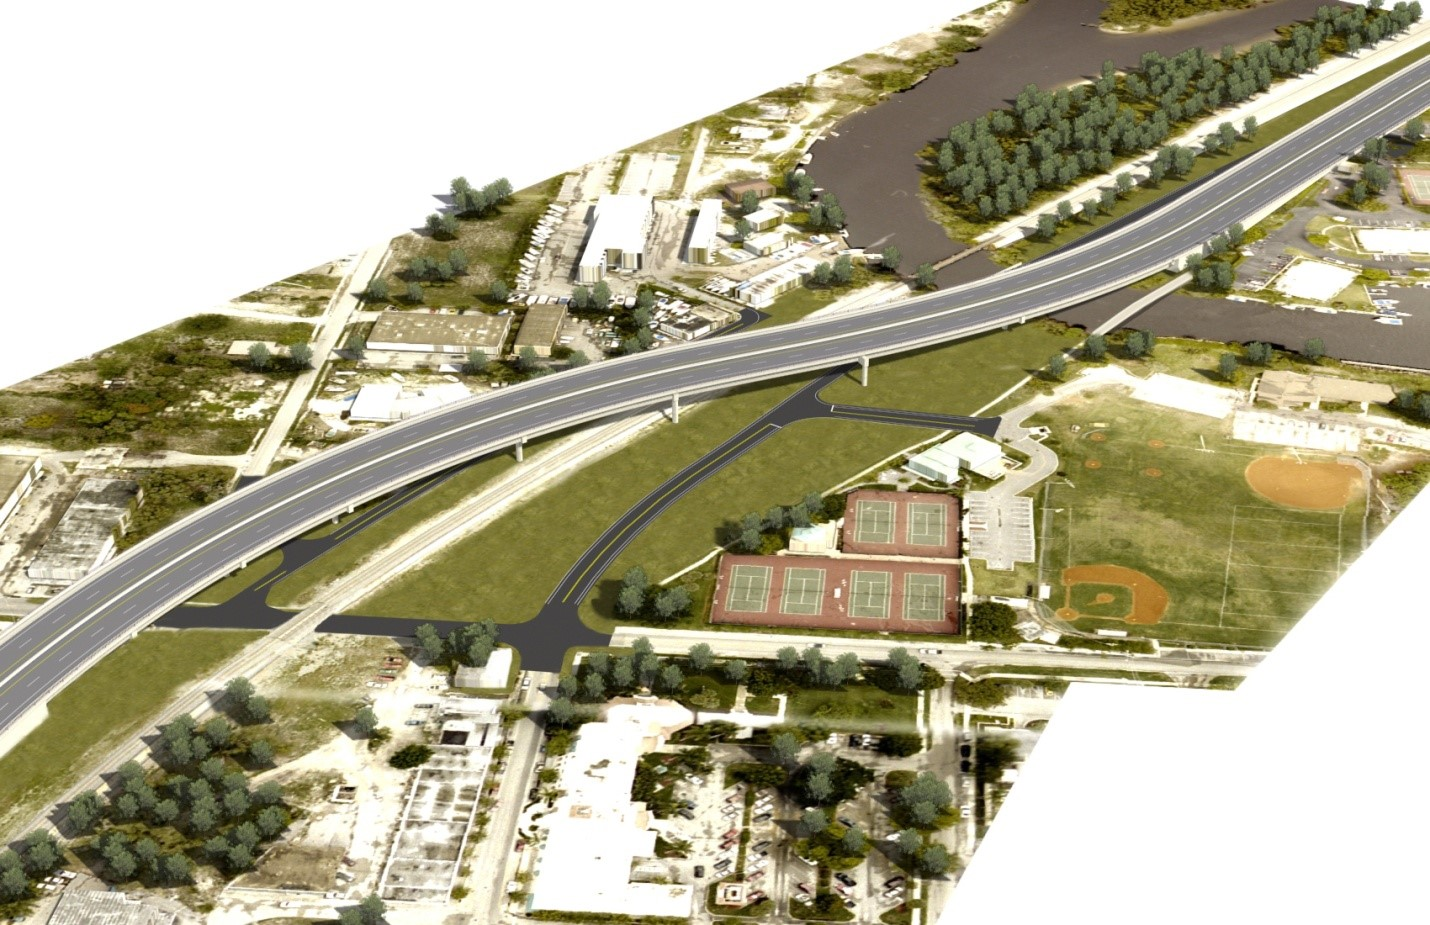
\includegraphics[width=\linewidth]{bridge-aerial.jpg}
  \caption{某桥梁项目的概念性鸟瞰图}
  \label{fig:bridge-aerial}
\end{figure}
\begin{figure}
  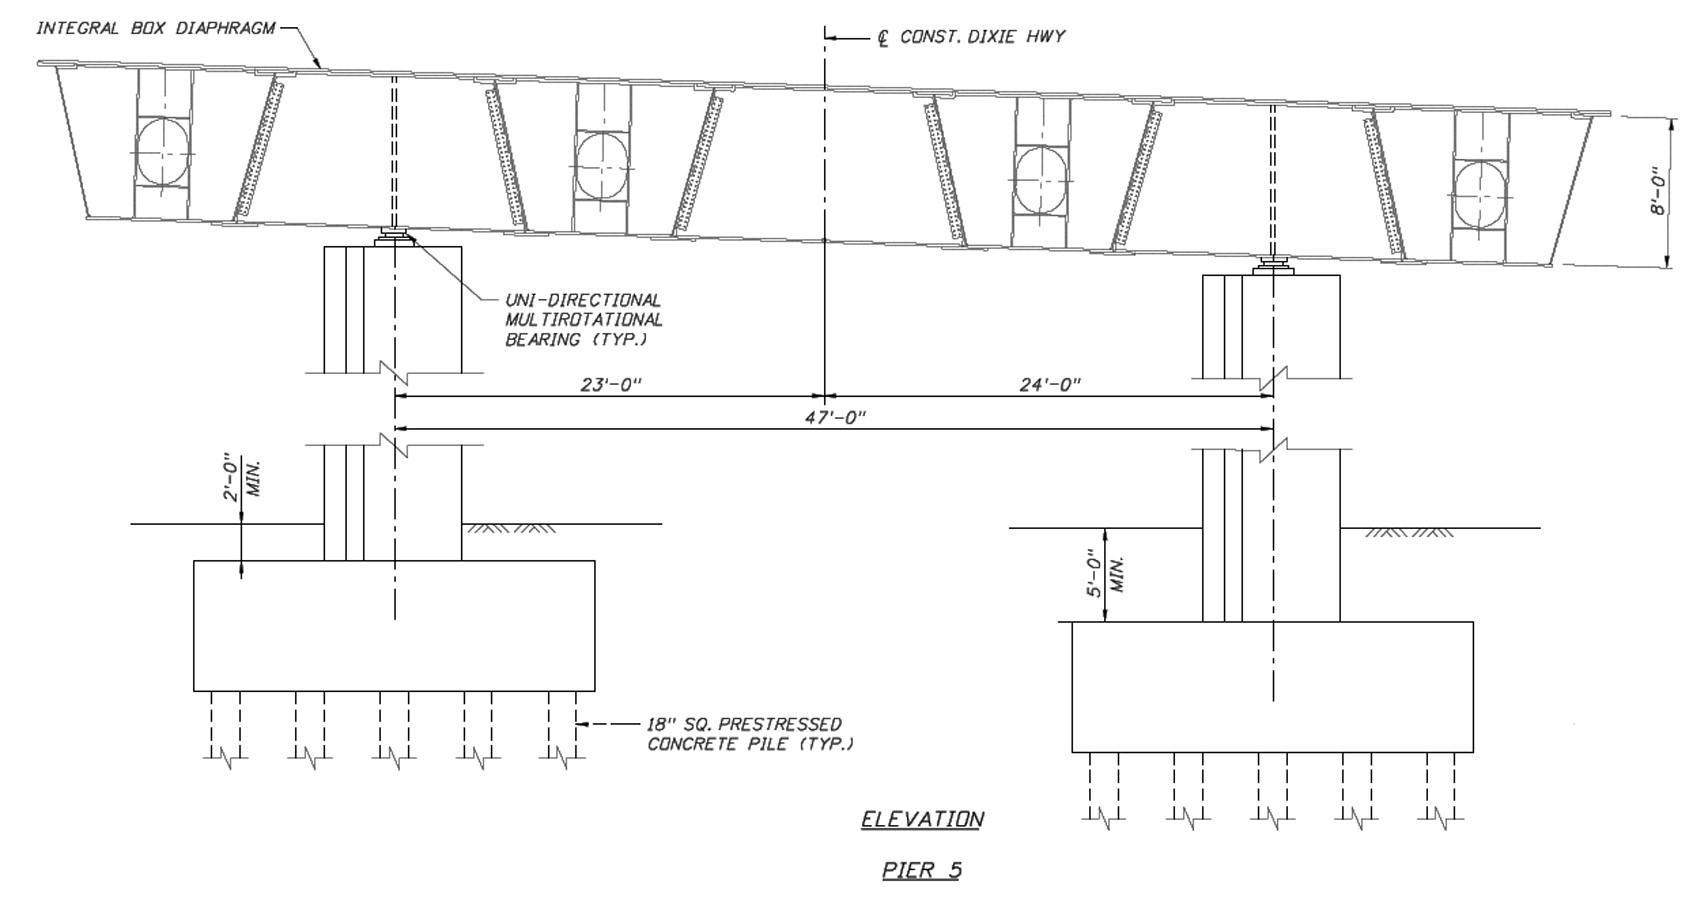
\includegraphics[width=\linewidth]{typical-section.jpg}
  \caption{典型的上部结构/下部结构布置}
  \label{fig:typical-section}
\end{figure}
\begin{figure}
  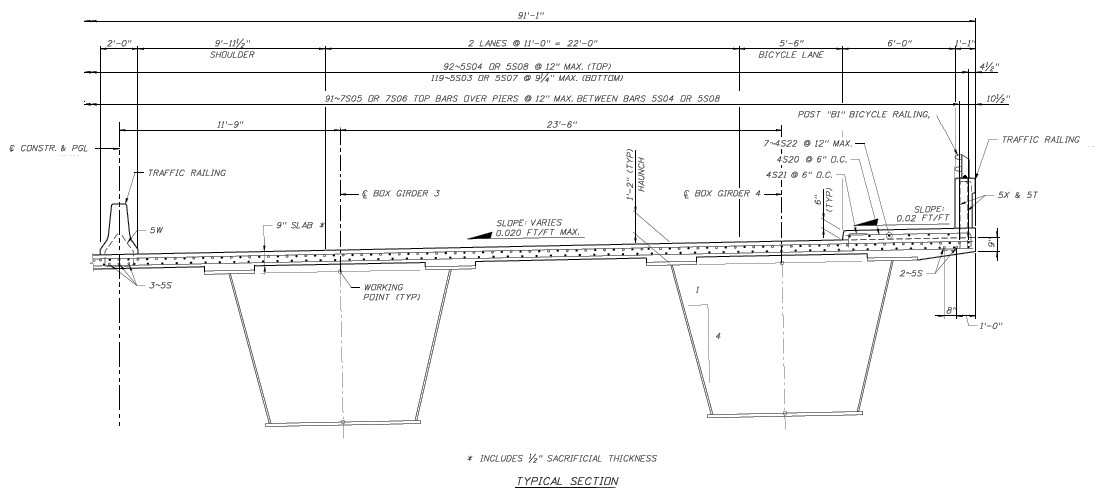
\includegraphics[width=\linewidth]{superstructure-section.jpg}
  \caption{上部结构截面——桥面——现浇方案,按 \lrfd 设计}
  \label{fig:superstructure-section}
\end{figure}

% The bridge setting includes the following characteristics, which have an influence on the service life:
桥梁的以下特性对\gls*{servicelife}有影响:
\begin{itemize}
  % \item Located in a cold environment where deicing salts are utilized, and multiple cycles of freeze/thaw are anticipated;
  \item 桥梁位于使用除冰盐的寒冷环境中,预计会有多次冻融循环;
  % \item Located in an area where studded tires are used in the winter;
  \item 桥梁位于冬季使用镶钉轮胎的区域;
  % \item Subjected to potential overloads with 20-kip tire loads in an HL93 truck configuration;
  \item 轮重 \qty{90}{kN} 的 HL93 型重载卡车引起潜在的超载;
  % \item Spans over a navigable waterway with primarily brackish conditions, and located adjacent to a park with water access for jet skis;
  \item 桥梁横跨主要为微咸水水质的通航航道,并毗邻一个公园,公园内有供水上摩托艇使用的航道;
  % \item Located near the coastline with possible salt water storm surge with potential hurricane force winds up to 150 mph wind gusts; and
  \item 桥梁位于海岸线附近,可能有咸水风暴潮,潜在飓风强度可达 \qty{240}{km/h};
  % \item Located in an area where local aggregates are subject to ASR.
  \item 桥址所在区域,当地的混凝土骨料材料会受到\acrfull{asr}影响。
\end{itemize}


% \subsection{Steps in Addressing Service Life Design}
\subsection{解决使用寿命设计的步骤}
% The first step in the process for addressing the service life design issue for bridge deck is to follow the flowchart shown in Section 4.5 of the Guide and repeated in \cref{fig:flowchart-guide}
解决桥面板\gls*{servicelife}设计问题的第一步是遵循\bkn{指南}\cref{sec:overall-strategy}中所示的流程图,此处于 \cref{fig:flowchart-guide} 重复列出。

\begin{figure}
  % \includegraphics[width=\linewidth]{graphic-file}
  \caption{\bkn{指南}\cref{chp:bridge-decks}所示流程图(\cref{fig:deck-selection-process})}\label{fig:flowchart-guide}
\end{figure}

% \cref{tab:operational-local-factors-considered} is used to extract the information needed to address the requirements of Steps 1a and 1b shown in \cref{fig:flowchart-guide}
\cref{tab:operational-local-factors-considered} 用于提取满足 \cref{fig:flowchart-guide} 中步骤 1a 和 1b 要求所需的信息。


\begin{table}
  \caption{要考虑的运营和当地因素——\cref{fig:flowchart-guide} 中的步骤 1a 和 1b}\label{tab:operational-local-factors-considered}
  % \input{tables/operational-local-factors-considered}
\end{table}

% The information shown in \cref{tab:operational-local-factors-considered} is developed from project requirements, and exemplifies the type of information necessary for layout and service life evaluation of the entire bridge system. It is well beyond that needed for simply evaluating a bridge deck, but is provided here for completeness. The pertinent issues in \cref{tab:operational-local-factors-considered}, with respect to the bridge deck, are indicated by an arrow at the right side of the table.
\cref{tab:operational-local-factors-considered} 中显示的信息是根据项目要求开发的,举例说明了整个桥梁{系统}的布局和{使用寿命}评估所需的信息类型。 它远远超出了简单评估桥面板所需的范围,但在此提供是为了完整性。 \cref{tab:operational-local-factors-considered} 中与桥面相关的相关问题在表格右侧用箭头表示。

% The next step is to identify the possible bridge deck alternatives, as indicated by Step 2 in \cref{fig:flowchart-guide}. Information provided in Section 2.3.2 of Chapter 2 and Section 4.2.1 of Chapter 4 of the Guide can be used to obtain advantages and disadvantages of various deck systems. In the case of major and complex bridges the designer may consider feasible bridge deck systems based on local preferences and experiences. In the current example, it is assumed that only the cast-in-place option is selected, as indicated in the typical girder cross section shown in Figure 1.16.
下一步是确定可能的桥面系备选方案,如\cref{fig:flowchart-guide} 中的步骤 2 所示。 本\bkn{指南}的\cref{chp:bridge-system-selection} \cref{subsec:factors-affect-deck}和第 4 章 的 4.2.1 节提供的信息可用于了解各种桥面系统的优缺点。 对于大型和复杂的桥梁,设计者可以根据当地的偏好和经验考虑可行的桥面系统。 在当前示例中,假设仅选择了现场浇筑选项,如\cref{fig:superstructure-section} 所示的典型梁横截面所示。

% Following are the steps shown in the flowchart given in Chapter 4, Section 4.4 of the Guide (Figure 4.19) and repeated in \cref{fig:flowchart-identify-factors} is the next step.
以下是\bkn{指南}\cref{chp:bridge-decks}\cref{sec:overall-strategy}(\cref{fig:mitigation-process})中给出的流程图中显示的步骤,并在 \cref{fig:flowchart-identify-factors} 重复列出。

\begin{figure}
  % \includegraphics[width=\linewidth]{graphic-file}
  % \caption{Flowchart to identify factors affecting service life. (Figure 4.19 of Guide)}
  \caption{确定影响使用寿命的因素的流程图(\bkn{指南}\cref{fig:mitigation-process}}
  \label{fig:flowchart-identify-factors}
\end{figure}

% \cref{fig:flowchart-identify-factors} aids in identifying factors that affect service life of bridge deck and in selecting possible strategies capable of mitigating the adverse effects of these factors. Identifying the factors that affect service life of bridge deck can be accomplished using the fault trees provided in \cref{chp:bridge-decks}, Section 4.2 of the Guide. Navigating through the fault tree can be simplified through the use of software. \cref{fig:screenshort} shows an example of what an Excel-based solution could look like. Using the software shown in \cref{fig:screenshort}, the user selects applicable factors from the first fault tree layer then continues through successive layers until reaching the last levels, which are depicted as circles. The items listed in each circle are the factors that will have to be addressed in the design for service life process. Each factor has the capability of reducing the service life of bridge deck. \cref{chp:bridge-decks} identifies one or more strategies capable of mitigating the effect of each particular factor listed in the circles.
\cref{fig:flowchart-identify-factors} 有助于识别影响桥面板\gls*{servicelife}的因素,并选择能够减轻这些因素不利影响的可能策略。 可以使用本\bkn{指南} \cref{chp:bridge-decks}\cref{sec:factors-influence}中提供的\gls*{faulttree}来确定影响桥面\gls*{servicelife}的因素。 通过使用软件可以简化\gls*{faulttree}的导航。 \cref{fig:screenshort} 显示了基于 \Excel\ 的解决方案的示例。 使用\cref{fig:screenshort} 中所示的软件,用户从第一个\gls*{faulttree}层选择适用的因素,然后继续通过后续层,直到到达最后一层,这些层被描绘为圆圈。 每个圆圈中列出的项目是在\gls*{servicelife}设计过程中必须解决的因素。 每个因素都有降低桥面板\gls*{servicelife}的能力。 \cref{chp:bridge-decks}确定了一种或多种能够减轻圆圈中列出的每个特定因素影响的策略。

\begin{figure}
  % \includegraphics[width=\linewidth]{graphic-file}
  \caption{Excel 工作表中\gls*{faulttree}导航的屏幕截图}\label{fig:screenshort}
\end{figure}

% \cref{fig:screenshort} shows branches of the fault tree that are applicable to the example under consideration. In the first layer, based on the project requirements, a decision is made that the service life of bridge deck can only be reduced due to deficiencies. The second layer states that either loads or natural or man-made hazards can cause bridge deck deficiencies. Both are judged to be applicable and are therefore selected. \cref{fig:screenshort} then shows the progression through the fault tree on the branch related to the factor, due to loads. The fourth layer in \cref{fig:screenshort} states that either traffic-induced loads or system-dependent loads can reduce service life of bridge deck. Again, both factors are judged to be applicable and the boxes are checked. Further, the reduction in service life of bridge deck as a result of traffic-induced loads can be caused by fatigue, overload, or wear, as depicted by the circles. All circles are applicable to the example. \cref{fig:screenshort} also identifies each factor that is capable of reducing the service life of bridge deck as a result of system-dependent loads, as shown in circles and identified as differential shrinkage, thermal, and system framing restraint. Based on project requirements, these factors are also judged applicable for consideration when addressing service life design.
\cref{fig:screenshort} 显示适用于正在考虑的示例的\gls*{faulttree}分支。第一层,根据工程要求,决定桥面因缺陷只能减少{使用寿命}。 第二层指出,负载或自然或人为的危害都可能导致桥面缺陷。 两者都被判断为适用,因此被选中。 \cref{fig:screenshort} 然后显示由于负载,\gls*{faulttree}在与该因素相关的分支上的进展。 \cref{fig:screenshort} 中的第四层指出,交通引起的负载或系统相关负载都会缩短桥面板的{使用寿命}。 同样,这两个因素都被判断为适用,并且复选框被选中。 此外,如圆圈所示,疲劳、过载或磨损可能导致交通荷载导致的桥面{使用寿命}缩短。 所有圆圈都适用于该示例。 \cref{fig:screenshort} 还确定了由于系统相关载荷而能够缩短桥面板{使用寿命}的每个因素,如圆圈所示,并确定为差异收缩、热和系统框架约束。 根据项目要求,这些因素也被判断为适用于在解决{使用寿命}设计时要考虑的因素。

% The circles in the fault tree signify:
\gls*{faulttree}中的圆圈表示:

\begin{itemize}
  \item 能够缩短使用寿命的问题;
  \item 设计者需要制定策略来缓解问题的问题。
\end{itemize}

% The strategies to address the individual items listed in each circle are provided in the Guide, in this case in Chapter 4 on bridge decks. It should also be noted that for most factors listed in the circles, the Guide identifies more than just one possible strategy.
指南中提供了解决每个圆圈中列出的各个项目的策略,在本例中是关于桥面的第 4 章。 还应注意的是,对于圆圈中列出的大多数因素,指南确定的不仅仅是一种可能的策略。

% To complete the process of navigating through the fault tree, all branches applicable to the problem need to be considered and applicable circles checked. Figure 1.20 shows the remainder of the fault tree with the “Due to Loads” branch collapsed for clarity. The decision for selecting the applicable circles is based on specific project conditions and requirements.
要完成通过\gls*{faulttree}导航的过程,需要考虑适用于问题的所有分支并检查适用的圈子。 \cref{fig:segment-fault-tree} 显示了\gls*{faulttree}的其余部分,为清楚起见,“由于负载”分支已折叠。 选择适用圈子是根据具体的项目条件和要求决定的。


\begin{figure}
  % \includegraphics[width=\linewidth]{graphic-file}
  \caption{示例中勾选了适用圆圈的\gls*{faulttree}片段}\label{fig:segment-fault-tree}
\end{figure}

% \subsection{Developing Strategies and Alternative Solutions}
\subsection{制定战略和备选解决方案}

% Once the fault tree is completed and all applicable factors are identified, the individual strategies capable of mitigating the factors can be collected. If software is utilized to work through the fault tree then this step can be automated based on the selections made. \cref{tab:mitigate-factors-strategy} summarizes the list of individual strategies capable of mitigating the factors developed for the example problem as identified as checked circles in \cref{fig:screenshort,fig:segment-fault-tree}.
一旦\gls*{faulttree}完成并确定了所有适用因素,就可以收集能够减轻这些因素的个别策略。如果使用软件来处理\gls*{faulttree},则可以根据所做的选择自动执行此步骤。\cref{tab:mitigate-factors-strategy} 总结了能够减轻为示例问题开发的因素的单个策略列表,这些因素在 \cref{fig:screenshort,fig:segment-fault-tree} 中被标识为选中的圆圈。

\begin{table}
  \caption{能够减轻影响示例问题使用寿命的因素的个别策略列表}\label{tab:mitigate-factors-strategy}
  % \input{tables/filename}
\end{table}

% At this point, the designer has developed a complete list of strategies that can be used for mitigating various factors capable of affecting the service life of bridge deck, based on project requirements. \cref{tab:mitigate-factors-strategy} also provides sections of the Guide that the user can refer to for more information, and lists advantages and disadvantages of the defined strategies. Some of the strategies may contradict each other while others may result in similar results. Intentionally, the Guide does not provide a single strategy or attempt to identify the best strategy. In many cases strategies to mitigate the individual factors capable of reducing service life are context sensitive, meaning that the best strategy is very much dependent on such factors as local practice, environment, or owner preferences.
至此,设计师已经根据项目要求制定了一份完整的策略清单,可用于缓解影响桥面板使用寿命的各种因素。 \cref{tab:mitigate-factors-strategy} 还提供了用户可以参考以获取更多信息的指南部分,并列出了已定义策略的优点和缺点。 一些策略可能相互矛盾,而另一些策略可能会产生相似的结果。 有意地,该指南不提供单一策略或尝试确定最佳策略。 在许多情况下,减轻能够缩短使用寿命的个别因素的策略是上下文敏感的,这意味着最佳策略在很大程度上取决于当地实践、环境或业主偏好等因素。

% As mentioned, some of the strategies may contradict each other and some may be more preferable based on local practices or owner preferences. Consequently, the next step for the designer is to select strategies that are desirable for each factor affecting the service life. \cref{tab:strategy-deck-alternatives} shows a narrower list of strategies extracted from the complete list given in \cref{tab:mitigate-factors-strategy}. The first row in \cref{tab:strategy-deck-alternatives} shows the applicable factors that can reduce the service life of bridge deck under consideration. These factors were obtained by navigating through branches of the fault tree.
如前所述,一些策略可能相互矛盾,而根据当地实践或所有者偏好,一些策略可能更可取。 因此,设计师的下一步是选择适合影响使用寿命的每个因素的策略。\cref{tab:strategy-deck-alternatives} 显示了从 \cref{tab:mitigate-factors-strategy} 中给出的完整列表中提取的更窄的策略列表。\cref{tab:strategy-deck-alternatives} 中的第一行显示了可能会缩短所考虑的桥面板使用寿命的适用因素。 这些因素是通过浏览\gls*{faulttree}的分支获得的。

\begin{table}
  \caption{桥面系备选方案专用策略列表}\label{tab:strategy-deck-alternatives}
  % \input{tables/filename}
\end{table}


% In developing the information shown in \cref{tab:strategy-deck-alternatives}, the designer may consider many factors and ensure that there are no contradicting strategies. For instance, appropriate concrete mix is specified as one strategy to address wear, differential shrinkage, freeze/thaw, humidity, and ASR/ACR. The designer must ensure that a concrete mix capable of addressing all of these issues can be developed. Otherwise, for a particular factor the designer may be forced to use another strategy. As an example for differential shrinkage, a low modulus of elasticity concrete is needed, whereas for wear, a high modulus of elasticity is needed. Consequently, to address wear and differential shrinkage, the same concrete mix cannot be used to mitigate both factors, and within a given deck alternative, one of these factors should be mitigated using a different strategy.
在开发 \cref{tab:strategy-deck-alternatives} 中显示的信息时,设计者可能会考虑许多因素并确保没有矛盾的策略。 例如,适当的混凝土混合物被指定为解决磨损、收缩差异、冻结/解冻、湿度和 ASR/ACR 的一种策略。 设计师必须确保能够开发出能够解决所有这些问题的混凝土组合。 否则,对于特定因素,设计者可能被迫使用另一种策略。 例如,对于不同的收缩,需要低弹性模量的混凝土,而对于耐磨,则需要高弹性模量。 因此,为了解决磨损和收缩差异,不能使用相同的混凝土混合物来减轻这两个因素,并且在给定的甲板替代方案中,应该使用不同的策略来减轻其中一个因素。

% The next step in the process is to develop possible deck alternatives that meet both LRFD Specifications requirements and Guide requirements.
该过程的下一步是开发满足 \lrfd 要求和\bkn{指南}要求的可能桥面系备选方案。

% Using the information provided in \cref{tab:strategy-deck-alternatives} and ensuring there is no contradiction among strategies to mitigate various factors, \cref{tab:alternative-aashto-guide} shows four possible deck alternatives capable of mitigating all factors affecting the service life of the bridge for the example under consideration. The four alternatives shown in \cref{tab:alternative-aashto-guide} are project specific solutions. It is also possible to automate this step by first identifying all possible deck alternatives based on all possible combinations of strategies listed in \cref{tab:strategy-deck-alternatives} and then eliminating those judged not feasible, because of contradiction among strategies.
使用 \cref{tab:strategy-deck-alternatives} 中提供的信息并确保减轻各种因素的策略之间没有矛盾,\cref{tab:alternative-aashto-guide} 显示了四种可能的套牌替代方案,能够减轻所有因素 影响正在考虑的例子中桥梁的使用寿命。 \cref{tab:alternative-aashto-guide} 中显示的四个备选方案是项目特定的解决方案。 也可以通过首先根据 \cref{tab:strategy-deck-alternatives} 中列出的所有可能的策略组合识别所有可能的套牌替代方案,然后消除那些由于策略之间的矛盾而被判断为不可行的套牌替代方案,从而自动执行此步骤。

\begin{table}
  \caption{开发同时满足 \acrshort{aashto} 和\bkn{指南}要求的桥面系备选方案}\label{tab:alternative-aashto-guide}
  % \input{tables/filename}
\end{table}


% For each alternative shown in \cref{tab:alternative-aashto-guide}, rows two through 11 show the service life design factors identified in \cref{tab:strategy-deck-alternatives} and corresponding strategies selected for each alternative. Incorporating all of the select strategies listed in rows 2 through 11 for each of the four alternatives results in modified deck configurations shown in row 13 of \cref{tab:alternative-aashto-guide}. Development of the four deck alternatives signifies the completion of step 4a shown in \cref{fig:flowchart-identify-factors}. It should be mentioned that strategies listed in \cref{tab:strategy-deck-alternatives} could lead to the development of additional deck alternatives. However, for the sake of simplicity, only four alternatives are shown in \cref{tab:alternative-aashto-guide}.
对于 \cref{tab:alternative-aashto-guide} 中显示的每个备选方案,第 2 行到 11 行显示了 \cref{tab:strategy-deck-alternatives} 中确定的使用寿命设计因素以及为每个备选方案选择的相应策略。 将第 2 行到第 11 行中列出的所有选择策略合并到四个备选方案中的每一个,会导致修改后的套牌配置,如 \cref{tab:alternative-aashto-guide} 的第 13 行所示。 四副套牌替代品的开发标志着 \cref{fig:flowchart-identify-factors} 中所示的步骤 4a 的完成。 应该提到的是,在 \cref{tab:strategy-deck-alternatives} 中列出的策略可能会导致开发额外的套牌替代方案。 然而,为了简单起见,\cref{tab:alternative-aashto-guide} 中只显示了四个备选方案。


% The first option shown in \cref{tab:alternative-aashto-guide}, column 2, represents a design that meets the strength requirements stated in LRFD Specifications. The total deck thickness is 8 in., with no considerations for any of the factors capable of reducing the service life. The main feature of the first alternative, Alt. 1 in \cref{tab:alternative-aashto-guide}, is having impermeable concrete, with 5\% silica fume and 10\% fly ash. The addition of fly ash is assumed to impact the rate of reduction in the diffusivity of concrete, a parameter used in estimating the time to initiate corrosion.
\cref{tab:alternative-aashto-guide} 第 2 列中显示的第一个选项表示满足 LRFD 规范中规定的强度要求的设计。 甲板总厚度为 8 英寸,未考虑任何可能缩短使用寿命的因素。 第一个替代方案的主要特征,Alt。 \cref{tab:alternative-aashto-guide} 中的 1,具有防渗混凝土,含 5\% 硅粉和 10\% 粉煤灰。 假设添加飞灰会影响混凝土扩散系数的降低速率,这是用于估计开始腐蚀时间的参数。

% The second alternative, Alt. 2 in \cref{tab:alternative-aashto-guide}, relies mainly on the use of stainless steel reinforcement, in this case Grade 316 stainless steel, to prevent corrosion. Alternative 3, Alt. 3 in \cref{tab:alternative-aashto-guide}, uses regular concrete with increased cover to delay the time to initiate the corrosion. Finally, the fourth alternative, Alt. 4 in \cref{tab:alternative-aashto-guide}, uses a membrane and overlay to address corrosion.
第二种选择,Alt。 \cref{tab:alternative-aashto-guide} 中的 2,主要依靠使用不锈钢加固,在本例中为 316 级不锈钢,以防止腐蚀。 备选方案 3,备选方案。 3 在 \cref{tab:alternative-aashto-guide} 中,使用增加覆盖层的普通混凝土来延迟开始腐蚀的时间。 最后,第四种选择,Alt。 \cref{tab:alternative-aashto-guide} 中的 4,使用膜和覆盖层来解决腐蚀问题。

% All alternatives use increased thickness to address overload, increasing the deck thickness by 0.5 in. \cref{tab:alternative-aashto-guide} also addresses additional strategies capable of reducing service life of the various alternatives.
所有备选方案都使用增加厚度来解决过载问题,将甲板厚度增加 0.5 英寸。\cref{tab:alternative-aashto-guide} 还解决了能够缩短各种备选方案使用寿命的其他策略。


% \subsection{Evaluating Alternatives}
\subsection{评估备选方案}
% As shown in \cref{fig:flowchart-guide}, the next step is predicting the service life of each alternative, Step 5 in \cref{fig:flowchart-guide}, and comparing it to the design service life of the bridge system, as specified by the owner and project requirements. Based on the outcome, the development of rehabilitation or replacement requirements, Step 5a in \cref{fig:flowchart-guide}, and a maintenance plan, Step 6 in \cref{fig:flowchart-guide}, may be necessary. The last step for the bridge deck alternative under consideration, as shown in \cref{fig:flowchart-guide}, Step 7, is to perform life cycle cost analysis for comparison.
如 \cref{fig:flowchart-guide} 所示,下一步是预测每个备选方案的使用寿命,\cref{fig:flowchart-guide} 中的第 5 步,并将其与桥梁系统的设计使用寿命进行比较 ,由业主和项目要求指定。 根据结果,可能需要制定修复或更换要求(\cref{fig:flowchart-guide} 中的步骤 5a)和维护计划(\cref{fig:flowchart-guide} 中的步骤 6)。如 \cref{fig:flowchart-guide} 第 7 步所示,正在考虑的桥面板备选方案的最后一步是执行生命周期成本分析以进行比较。

% As described in \cref{chp:bridge-system-selection} on system selection, the designer must also consider the interaction that might exist between various parts of the bridge. This step is not covered for this example.
正如 \cref{chp:bridge-system-selection} 中关于\gls*{system}选择的描述,设计者还必须考虑桥梁各部分之间可能存在的相互作用。此示例不包括此步骤。

% The potential service life of each deck alternate can be calculated based on the assumption that the main mode of deterioration is ingress of chloride into concrete, which can result in corrosion of reinforcement. One approach is to use the solution to Fick's second law as shown below.
每个桥面系备选方案的潜在使用寿命可以基于以下假设来计算:主要的劣化模式是氯离子对混凝土的渗透,这会导致钢筋腐蚀。一种方法是使用菲克第二定律的解决方案,如下所示。

% In a one-dimensional case, Fick's Law can be expressed and illustrated as follows:
在一维情况下,菲克定律可以表达如下:
\begin{equation}
  \label{eq:ficks-law}
  C(x,t)=C_0\left(1- \erf \frac{x}{2\sqrt{D_\text{c}t}} \right)
\end{equation}
\begin{EqDesc}{C(x,t)}
  \item[C(x,t)] 深度 $x$ 处在时间 $t$ 时的氯离子浓度;
  \item[C_0] 表明氯离子浓度(\unit{kg/m^3});
  \item[D_\text{c}] 氯离子扩散常数(\unit{cm^2/yr});
  \item[\erf] 误差函数(来自标准数学表)。
\end{EqDesc}

% The use of Fick's Law to determine the time of corrosion initiation is described in \cref{chp:corrosion-of-steel-rc-bridge}\cref{sec:description-corrosion}, of the Guide. \cref{eq:ficks-law} can be used to assess ingress of chloride through the concrete cover. As an example, \cref{fig:chloride-concentration} indicates the type of information that can be developed, which shows chloride concentration through the deck thickness for three time periods, after a deck is cast.
本指南的\cref{chp:corrosion-of-steel-rc-bridge}\cref{sec:description-corrosion}中描述了使用菲克定律确定腐蚀开始时间。\cref{eq:ficks-law} 可用于评估氯离子通过混凝土保护层的侵入。例如,\cref{fig:chloride-concentration} 表示可以开发的信息类型,它显示了桥面板浇筑后三个时间段内整个桥面板厚度中的氯离子浓度。

\begin{figure}
  % \includegraphics[width=\linewidth]{graphic-file}
  \caption{混凝土中的氯化物浓度与时间的关系}\label{fig:chloride-concentration}
\end{figure}

% The information shown in \cref{fig:chloride-concentration} can be used to predict the time when corrosion will be initiated, which in turn can be used to estimate the service life of the bridge deck, if corrosion of reinforcement is the main mode of deterioration. The Fick's law in this case is the deterioration model.
\cref{fig:chloride-concentration} 中显示的信息可用于预测腐蚀开始的时间,如果钢筋腐蚀是主要模式,这又可用于估计桥面板的使用寿命 的恶化。 这种情况下的菲克定律是退化模型。

% To complete the example, Life-365, a free program developed by the concrete industry, is used to conduct the life cycle cost analysis and assist in selecting an optimum solution. Life-365 uses a finite-difference approach to solve Fick's second law and to estimate the time to initiation of corrosion. Other approaches such as error function solution to Fick's second law, \cref{eq:ficks-law}, could also be used.
为了完成这个例子,\gls{life365} 是一个由混凝土行业开发的免费程序,用于进行生命周期成本分析并协助选择最佳解决方案。 \gls{life365} 使用有限差分法求解菲克第二定律并估计腐蚀开始的时间。也可以使用其他方法,例如菲克第二定律的误差函数解法 \cref{eq:ficks-law}。

% The solution to Fick's second law estimates the time to initiation of corrosion, $t_\text{i}$. For the example, it is assumed (assumption within Life-365) that once the corrosion is initiated, the time to propagate the corrosion to the point at which repair is needed, $t_\text{r}$ , is a constant six years, regardless of concrete mix used. Following the time period, $t_\text{i} + t_\text{r}$, Life-365 assumes repair action at set time intervals, say every 10 or 20 years, and set cost per unit area in square feet. Further, within each repair cycle, it is assumed that only a portion of the deck area will be repaired. For instance, within each repair cycle only 10\% or 20\% of the deck will need repair.
菲克第二定律的解估计了腐蚀开始的时间 $t_\text{i}$。 例如,假设(\gls{life365} 中的假设)一旦腐蚀开始,腐蚀传播到需要修复的点的时间 $t_\text{r}$ 是恒定的六年 , 无论使用何种混凝土混合物。 在时间段 $t_\text{i} + t_\text{r}$ 之后,\gls{life365} 会按设定的时间间隔(比如每 10 年或 20 年)采取维修行动,并设定单位面积的成本(以平方英尺为单位)。 此外,在每个维修周期内,假设只有一部分甲板区域将被维修。 例如,在每个维修周期内,只有 10\% 或 20\% 的甲板需要维修。

% The time to initiate corrosion depends on concrete mix and preventive measures, such as use of stainless steel, concrete cover, or membranes. Life-365 follows the guidance and terminology in ASTM E-917 Standard Practice for Estimating the Life Cycle Cost of Building System. The final number that can be used to select the optimal deck alternative can be the life cycle cost, which is the initial cost plus the present value of all future rehabilitation costs over the desired service life, in this case 100 years.
开始腐蚀的时间取决于混凝土混合料和预防措施,例如使用不锈钢、混凝土覆盖层或膜。 \gls{life365} 遵循 ASTM E-917 建筑系统生命周期成本估算标准实践中的指导和术语。 可用于选择最佳甲板备选方案的最终数字可以是生命周期成本,即初始成本加上预期使用寿命(在本例中为 100 年)内所有未来修复成本的现值。

% \cref{tab:input-parameters} shows the input parameters used within \gls{life365} to conduct a life cycle cost analysis for each of the four alternatives shown in \cref{tab:alternative-aashto-guide}.
\cref{tab:input-parameters} 显示了 \gls{life365} 中使用的输入参数,用于对 \cref{tab:alternative-aashto-guide} 中显示的四种备选方案中的每一种进行生命周期成本分析。

\begin{table}
  \caption{\gls{life365}中所有四种备选方案的输入参数}\label{tab:input-parameters}
  % \input{tables/filename}
\end{table}

% It is assumed that the bridge is located in Boston, Massachusetts; has a required service life of the deck of 100 years; and, for the sake of comparison, a total surface area of the deck of 10,000 square ft. \cref{tab:input-parameters} also shows the yearly temperature profile used. The diffusion coefficient and ingress of chloride are influenced by temperature fluctuation. The input parameters shown in \cref{tab:input-parameters} are applicable to all four alternatives shown in \cref{tab:alternative-aashto-guide}. The specific input and end results for each alternative are shown in \cref{tab:parameter-each-alternative}.
假设这座桥位于马萨诸塞州的波士顿;要求甲板的使用寿命为100年;并且,为了进行比较,甲板的总表面积为 10,000 平方英尺。\cref{tab:input-parameters} 还显示了所使用的年度温度曲线。扩散系数和氯化物的进入受温度波动的影响。\cref{tab:input-parameters} 中显示的输入参数适用于\cref{tab:alternative-aashto-guide} 中显示的所有四个备选方案。每个备选方案的具体输入和最终结果显示在\cref{tab:parameter-each-alternative} 中。

\begin{table}
  % \caption{Parameters Specific to Each Alternative}
  \caption{每个备选方案特定的参数}
  \label{tab:parameter-each-alternative}
  % \input{tables/filename}
\end{table}

% As indicated in \cref{tab:parameter-each-alternative}, alternatives 1, 2, 3, and 4 use the same concrete mix, hereafter referred to as regular mix, which was used for the base option designed in accordance with LRFD Specifications (option designated as AASHTO Design in \cref{tab:alternative-aashto-guide}). Alternative 1 uses 5\% silica fume to make the concrete impermeable. Alternative 2 uses stainless steel. Alternative 3 uses increased concrete cover to delay the adverse effects of corrosion. Alternative 4 uses a membrane and overlay.
如 \cref{tab:parameter-each-alternative} 所示,备选方案 1、2、3 和 4 使用相同的混凝土配合比,以下称为常规配合比,用于根据 LRFD 规范设计的基础选项 (在 \cref{tab:alternative-aashto-guide} 中指定为 AASHTO 设计的选项)。 备选方案 1 使用 5\% 硅粉使混凝土不透水。 备选方案 2 使用不锈钢。 备选方案 3 使用增加的混凝土保护层来延迟腐蚀的不利影响。 备选方案 4 使用薄膜和覆盖层。

% Following is a brief description of the results for each alternative.
以下是对每个备选方案的结果的简要说明。


% \paragraph*{Deck Design Based on LRFD Specifications}
\paragraph*{基于 \lrfd 的桥面板设计}
% As shown in \cref{tab:parameter-each-alternative}, in the case of the AASHTO base design, corrosion starts after 6.6 years (shown as Initiation). Thereafter, the propagation of corrosion to the point of needed repair is 6 years. At the end of 12.6 years, the repair and maintenance actions are assumed to start and continue every 10 years, during which 20\% of the surface area is repaired. These assumptions are used for the sake of demonstration and will vary based on various DOT preferences and practices. \cref{fig:total-life-cost} shows the total life cycle cost based on present value.
如 \cref{tab:parameter-each-alternative} 所示,在 \gls{aashto} 基础设计的情况下,腐蚀在 6.6 年后开始(显示为初始)。 此后,腐蚀传播到需要修复的点为 6 年。 在 12.6 年末,假设维修和保养行动每 10 年开始并持续一次,期间维修 20\% 的表面积。 这些假设用于演示目的,并且会根据各种 DOT 偏好和实践而有所不同。 \cref{fig:total-life-cost} 显示基于现值的总生命周期成本。

\begin{figure}
  % \includegraphics[width=\linewidth]{graphic-file}
  \caption{基于 \acrshort{lrfd} 规范的设计的总生命周期成本}\label{fig:total-life-cost}
\end{figure}

% The total life cycle cost for the AASHTO based design is \$774,676, which is shown in the last row of \cref{tab:parameter-each-alternative}. An inflation rate of 1.6\% and a discount rate of 2\% were used in developing the total life cycle cost. As indicated in \cref{tab:parameter-each-alternative}, the initial cost of AASHTO base design is the lowest of the alternatives (\$37, 215). However, the total life cycle cost is the highest (\$774,676). It should also be mentioned that these life cycle cost analyses ignore the user costs, or any other cost to society during repair and closure to traffic, and these costs can be significant.
基于 AASHTO 的设计的总生命周期成本为 774,676 美元,显示在 \cref{tab:parameter-each-alternative} 的最后一行。 计算总生命周期成本时使用了 1.6\% 的通货膨胀率和 2\% 的贴现率。 如 \cref{tab:parameter-each-alternative} 所示,AASHTO 基础设计的初始成本是所有备选方案中最低的 (\$37, 215)。 但是,总生命周期成本最高(\$774,676)。 还应该提到的是,这些生命周期成本分析忽略了用户成本,或在维修和关闭交通期间对社会造成的任何其他成本,这些成本可能是巨大的。


% \paragraph*{Alternative 1}
\paragraph*{备选方案 1}
% This alternative uses impermeable concrete by incorporating 5\% silica Fume in the mix. As a result, the initial unit cost of concrete is assumed to increase by ten dollars per cubic yard. The initiation of corrosion starts at 34.8 years after casting and the propagation phase lasts six years. Therefore, after 40.8 years the repair procedure is assumed to stat. It is assumed that the repair procedure is to be conducted every 10 years and during each repair cycle, 10\% of the surface area is assumed to need repair. Other repair alternatives can consist of complete replacement of deck every 40 years. The total life cycle cost of Alternative 1 for the assumptions made is \$277, 550, as shown in \cref{tab:parameter-each-alternative}. The initial cost of Alternative 1, \$44,645, is slightly higher than initial cost for AASHTO base design (\$37,215).
该替代方案通过在混合物中加入 5\% 硅粉来使用不透水混凝土。 因此,假设混凝土的初始单位成本每立方码增加 10 美元。 腐蚀开始于铸造后 34.8 年,传播阶段持续 6 年。 因此,在 40.8 年后,修复程序被假定为 stat。 假定维修程序每 10 年进行一次,并且在每个维修周期内,假定 10\% 的表面积需要维修。 其他维修方案包括每 40 年完全更换一次甲板。 如 \cref{tab:parameter-each-alternative} 中所示,根据所做的假设,备选方案 1 的总生命周期成本为 277 美元、550 美元。 备选方案 1 的初始成本为 44,645 美元,略高于 AASHTO 基础设计的初始成本(37,215 美元)。

% \paragraph*{Alternative 2}
\paragraph*{备选方案 2}
% This alternative uses Grade 316 stainless steel to address the corrosion of reinforcement issue. The time to initiation of corrosion for this alternative is more than 100 years and consequently no repair action is needed. The initial cost of using stainless steel is the highest among all alternatives (\$152,753). However, the total life cycle cost associated with Alternative 2, \$152,753 as shown in \cref{tab:parameter-each-alternative}, is the lowest among all alternatives.
该替代方案使用 316 级不锈钢来解决钢筋腐蚀问题。 这种替代品的腐蚀开始时间超过 100 年,因此不需要采取任何修复措施。 使用不锈钢的初始成本是所有替代品中最高的(\$152,753)。 然而,与备选方案 2 相关的总生命周期成本为 \cref{tab:parameter-each-alternative} 中所示的 \$152,753,是所有备选方案中最低的。

% \paragraph*{Alternative 3}
\paragraph*{备选方案 3}

% This alternative uses increased cover to delay the initiation of corrosion. Using increased cover delays the corrosion initiation from for AASHTO base design from 6.6 years to 15.2 years, as indicated in \cref{tab:parameter-each-alternative}. The total cost of Alternative 3 is relatively high, \$691,114. There does not seem to be much benefit in using this alternative, especially considering that increasing the concrete cover will subject the substructure and foundations to higher dead loads.
该替代方案使用增加的覆盖层来延迟腐蚀的开始。 使用增加的覆盖层可将 AASHTO 基础设计的腐蚀起始时间从 6.6 年延迟到 15.2 年,如 \cref{tab:parameter-each-alternative} 中所示。 备选方案 3 的总成本相对较高,为 \$691,114。 使用这种替代方案似乎没有太大好处,特别是考虑到增加混凝土保护层会使下部结构和地基承受更高的恒载。


% \paragraph*{Alternative 4}
\paragraph*{备选方案 4}

% Alternative 4 uses a membrane and overlay to prevent corrosion of reinforcement. The total deck thickness is only 8.5 in. compared to 9 in. and 10 in. used for Alternatives 1, 2 and 3. The repair cost per square foot for this alternative is assumed to be lower at \$20/ft2 as compared to \$50/ft2 for others when a membrane is used. It is assumed that a high quality membrane at \$7/ft2 is used and that it will last 75 years. Consequently, the repair will involve replacing damaged overlay areas, which are assumed to be 5\% of the total surface area during each repair cycle—every 10 years after 28.4 years of first installation (see \cref{tab:parameter-each-alternative}). At \$172,252, the total life cycle cost of this alternative, using membrane, is very low, while the initial cost (\$39,541 + \$70,000) is more than twice the AASHTO base design of \$37,215. It should also be mentioned that the use of a membrane could be much more economical than that indicated by this example. For instance, the calculation leads to the conclusion that corrosion will start after 28.4 years, which is not realistic. The concrete deck below the membrane could last a long time without any need for repair, and any needed repair action would only be for replacing the thin overlay, which could be achieved quickly with minimal interruption to traffic. These factors are not considered in conducting the life cycle cost analysis for this alternative.
备选方案 4 使用薄膜和覆盖层来防止钢筋腐蚀。 与备选方案 1、2 和 3 所用的 9 英寸和 10 英寸相比,总甲板厚度仅为 8.5 英寸。与 \ 使用膜时,其他人为 50 美元/平方英尺。 假设使用了 7 美元/平方英尺的高质量膜,并且它将持续 75 年。 因此,维修将涉及更换损坏的覆盖区域,假设在每个维修周期中更换损坏的覆盖区域 - 在首次安装 28.4 年后每 10 年更换一次(参见 \cref{tab:parameter-each-alternative}). 这种使用膜的替代方案的总生命周期成本为 172,252 美元,非常低,而初始成本(39,541 美元 + 70,000 美元)是 AASHTO 基础设计 37,215 美元的两倍多。 还应该提到的是,使用膜可能比本例所示的更经济。 例如,计算得出28.4年后开始腐蚀的结论,这是不现实的。 膜下的混凝土桥面可以持续很长时间而无需维修,任何需要的维修行动只是更换薄的覆盖层,可以在交通中断最少的情况下快速完成。 在对该备选方案进行生命周期成本分析时未考虑这些因素。

% \subsection{Summary and Conclusion}
\subsection{总结与结论}
% The table below provides a summary of results for all alternatives. Using this information it is feasible to conclude that use of stainless steel or membrane plus overlay can provide the best economy.
\cref{tab:alternative-summary} 汇总了所有备选方案的结果。使用此信息可以得出结论,使用不锈钢或加设薄膜覆盖层可以提供最佳的经济性。

\begin{table}
  \caption{备选方案汇总}\label{tab:alternative-summary}
  \begin{tblr}{
  colspec={c X[l] Q[r,si={table-format=7.0}] Q[r,si={table-format=7.0}]},
  row{1}={c,bg=genfg,fg=white,font=\bfseries,guard}
}
备选方案 & 解决腐蚀的主要方法        & 初始成本(\$)& 全生命周期成本(\$)\\
\acrshort{aashto} 基本设计 & N/A     & 37215    & 774676          \\
 方案 1      & 使用硅粉的抗渗混凝土  & 44645    & 277550          \\
 方案 2      & 使用 316 号不锈钢     & 152753   & 152753          \\
 方案 3      & 增大混凝土保护层      & 46519    & 691114          \\
 方案 4      & 使用薄膜和覆盖层      & 109541   & 172252          \\
\end{tblr}
\end{table}

% \section{Future Development of the Guide}
\section{《指南》的未来发展}
% The Guide provides a general, comprehensive framework for designing new bridges and rehabilitating existing bridges for service life. The approach presented by the Guide is flexible and can be adapted as new information becomes available. The Guide also provides a platform for developing customized manuals by individual State DOTs or for developing a customized and systematic approach for service life design of major and complex bridges.
本\bkn{指南}为设计新建桥梁和修复既有桥梁的\gls{servicelife}提供了一个通用的综合框架。本\bkn{指南}提出的方法是灵活的,可以根据新信息的出现进行调整。本\bkn{指南}还提供了一个平台,供各州\acrlong{dot}开发定制手册,或为大型复杂桥梁的\gls{servicelife}设计开发定制的系统方法。

% Design for service life is a context sensitive problem and local agency practices and preferences are important. Customizing the Guide can be achieved by using the general framework outlined in these pages and incorporating strategies and solutions preferred by each DOT for factors affecting service life of their bridges.
\gls{servicelife}设计是一个语境敏感的问题,即,当地机构的做法和偏好很重要。可以通过使用这概述的一般框架并结合每个\gls{dot}首选的措施和解决方案来定制\bkn{指南},以解决影响其桥梁\gls{servicelife}的因素。

% One of the challenges in developing true service life design is the lack of reliable, available deterioration models that are based on either field data or laws of physics governing the deterioration. Several studies are underway to develop deterioration models for various bridge elements, components, and subsystems. Such information can be incorporated into the Guide as they become available. These models are needed to further develop reliable life cycle cost analysis.

开发真实\gls*{servicelife}设计的挑战之一是缺乏基于现场数据或控制\gls*{deterioration}的物理定律的可靠、可用的\gls*{deterioration}模型。目前正在进行多项研究,以开发各种桥梁\gls{element}、\gls{component}和\gls{subsystem}的\gls*{deterioration}模型。此类信息可在可用时纳入\bkn{指南}。需要这些模型来进一步开发可靠的生命周期成本分析。

% There is a need to develop specific life cycle cost analysis tools dedicated to bridges, with the ability to incorporate user costs where applicable. These tools must be flexible enough to allow incorporating new information and deterioration models as they become available.

需要开发专用于桥梁的特定生命周期成本分析工具,并能够在适用的情况下纳入用户成本。这些工具必须足够灵活,以便在新信息和\gls*{deterioration}模型可用时纳入其中。

% There is a further need to develop more comprehensive examples, which take into account the interaction between solutions that may seem appropriate for an individual bridge element, component, or subsystem when viewed in isolation, and yet are less than optimum when considering service life solutions for the combined bridge system.

还需要开发更全面的示例,这些示例考虑了解决方案之间的相互作用,这些解决方案在孤立地看时似乎适合于单个桥梁\gls{element}、\gls{component}或\gls{subsystem},但在考虑\gls{servicelife}解决方案时却不是最佳的联合桥梁\gls{system}。

% Finally, the significant amount of information provided in the Guide is time consuming to comprehend in its entirety. There is a need to automate the use of the Guide by developing tools that would facilitate navigating through all of the included information.

最后,\bkn{指南}中提供的大量信息需要花费大量时间才能完全理解。有必要通过开发有助于浏览所有包含信息的工具来自动使用\bkn{指南}。
